\documentclass[12pt]{article}%iopart

%%
%%  Use \documentclass[boxit]{JAC2003}
%%  to draw a frame with the correct margins on the output.
%%
%%  Use \documentclass[acus]{JAC2003}
%%  for US letter paper layout
%%

\usepackage{graphicx}
\usepackage{listings}
\usepackage{color}
\usepackage{amssymb,amsmath,pdfpages}
\usepackage{bm}


\definecolor{codegreen}{rgb}{0,0.6,0}
\definecolor{codegray}{rgb}{0.5,0.5,0.5}
\definecolor{codepurple}{rgb}{0.58,0,0.82}
\definecolor{backcolour}{rgb}{0.95,0.95,0.92}

\lstdefinestyle{mystyleh5}{
    backgroundcolor=\color{backcolour},
    commentstyle=\color{codegreen},
    keywordstyle=\color{magenta},
    numberstyle=\tiny\color{codegray},
    stringstyle=\color{codepurple},
    basicstyle=\footnotesize,
    breakatwhitespace=false,
    breaklines=true,
    captionpos=b,
    keepspaces=true,
    numbers=none,
    numbersep=5pt,
    showspaces=false,
    showstringspaces=false,
    showtabs=false,
    tabsize=2
}

\lstdefinestyle{mystyle}{
    backgroundcolor=\color{backcolour},
    commentstyle=\color{codegreen},
    keywordstyle=\color{magenta},
    numberstyle=\tiny\color{codegray},
    stringstyle=\color{codepurple},
    basicstyle=\footnotesize,
    breakatwhitespace=false,
    breaklines=true,
    captionpos=b,
    keepspaces=true,
    numbers=left,
    numbersep=5pt,
    showspaces=false,
    showstringspaces=false,
    showtabs=false,
    tabsize=2
}

\lstset{style=mystyleh5}

\linespread{1.3}

%\usepackage[a4paper,%total={145mm,220mm},
%top=20mm, left=40mm,bottom=40mm, right=25mm, includefoot]{geometry}

\begin{document}

\title{Puffin Manual}

\maketitle

\newpage

\tableofcontents

\newpage

\section{Introduction}

%The code Puffin\cite{puffin} is an FEL simulation code  - it is a so-called `unaveraged' FEL code, which has an enhanced resolution over that of more conventional averaged codes. It can model fast changes in both the electron beam and radiation temporal structure, and can model any frequency (limited by the Niquist condition) and electron energy.  The code has undergone many improvements and extended its functionality since the initial publication in \cite{puffin}. It no longer uses an external linear solver package, and some of the scaling has changed - see below. Before, only the electron beam was distributed in memory across MPI nodes - now both the field and the beam are stored and solved in parallel, enabling the modelling of extremely large systems.

%Puffin can now output data in hdf5 format, with VizSchema metadata added to allow visualization with \textit{e.g.} Visit on a cluster. Some visualization examples are shown below in figures \ref{bbd1} and \ref{bbd2}.



Puffin (Parallel Unaveraged Fel INtegrator) simulates a Free Electron Laser (FEL). Puffin is a massively parallel numerical solver for an unaveraged, 3D FEL system of equations, and is written mostly in Fortran 90, using MPI and OpenMP.

The initial publication describing the first version of the code is in \cite{puffin}. The code has undergone many improvements and extended its functionality since then. It no longer uses an external linear solver package, and the only external package now required is FFTW v3.3.x onwards.

Puffin is a so-called 'unaveraged' FEL code - meaning it is absent of the slowly varying envelope approximation (SVEA) and wiggler period averaging approximations. It does not utilize a 'slicing' model of the beam phase space and radiation field, and instead utilizes an algorithm which is much more similar to a Particle-In-Cell (PIC) code methodology.

In addition, some accelerator components are included for simulation of the 'realistic' undulator line, and together with the lack of restrictions, means it may model:

\begin{itemize}
\item The full, broad bandwidth frequency spectrum, limited only by the Niquist frequency of the mesh
\item Full electron beam transport
\item Transport of large energy spread beams through the undulator, and the radiation emitted from these beams
\item Tapered undulators
\item Fully 3D undulators, including modelling of the wiggler entries/exits and natural focusing
\item Interleaved undulator-chicane lattices
\item Variably polarized undulators
\item Tuning of each undulator module
\end{itemize}

It presently does not include the effects of space charge, and ignores emission of the backwards wave from the e-beam.

\begin{figure*}
\centering
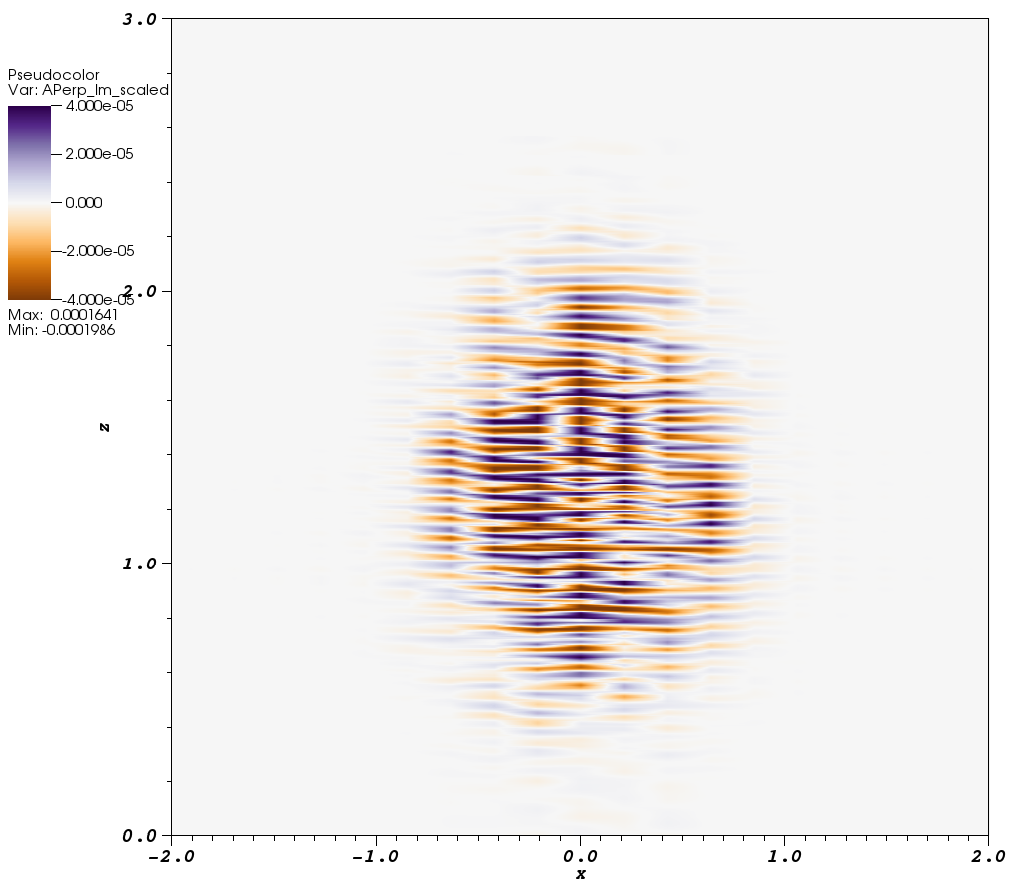
\includegraphics[width=60mm]{visit0032.png}
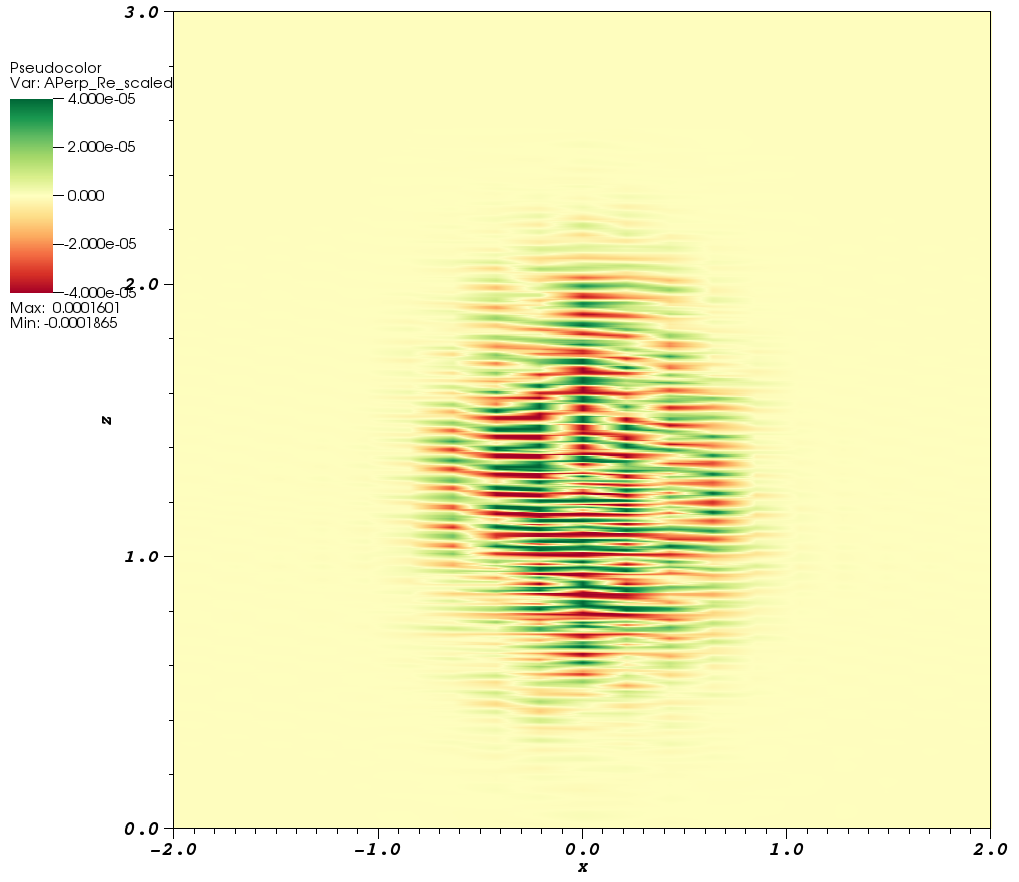
\includegraphics[width=60mm]{visit0033.png}
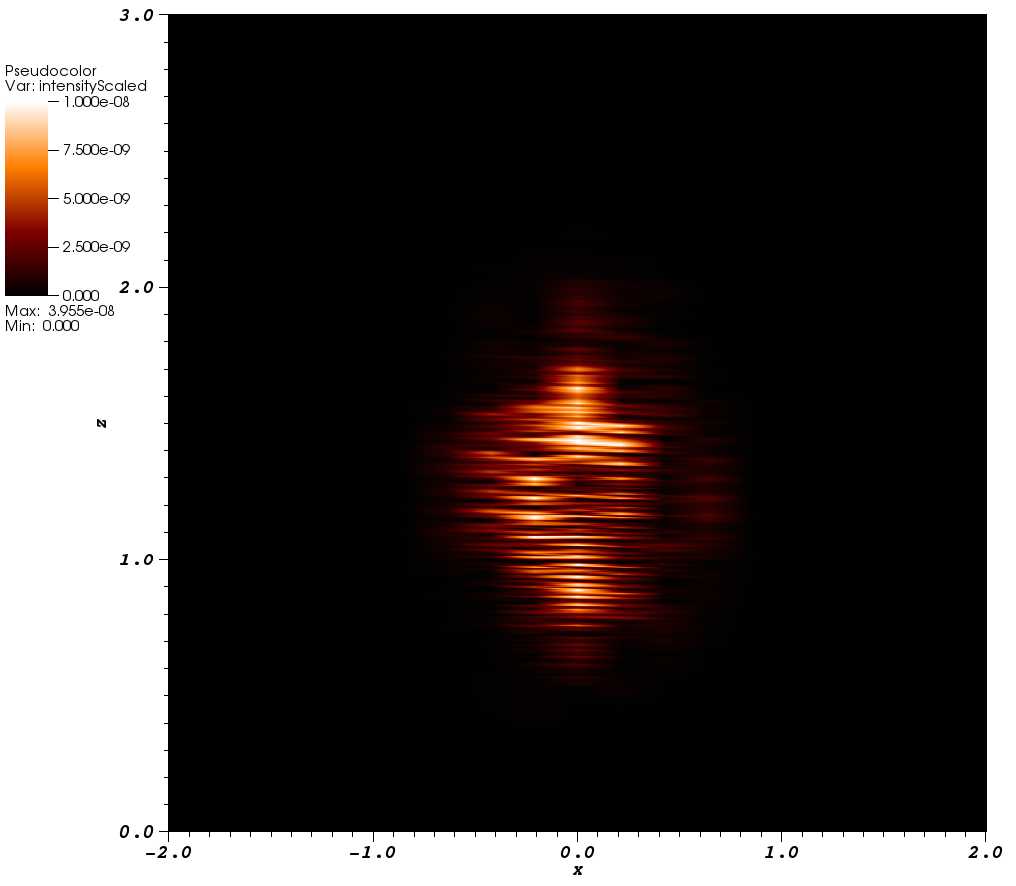
\includegraphics[width=100mm]{visit0035.png}
\caption{Radiated spontaneous field from Puffin in the first few undulator periods - $x$ (top left) and $y$ (top right) polarized fields, and instantaneous intensity (bottom), at $y=0$. Radiation is propagating in the negative $z$ direction (the vertical axis). One can see the noisy phase of the radiation in both transverse (x) and temporal (z) directions, which is due to the shot-noise of the electron beam.  }
\label{bbd1}
\end{figure*}




\begin{figure*}
\centering
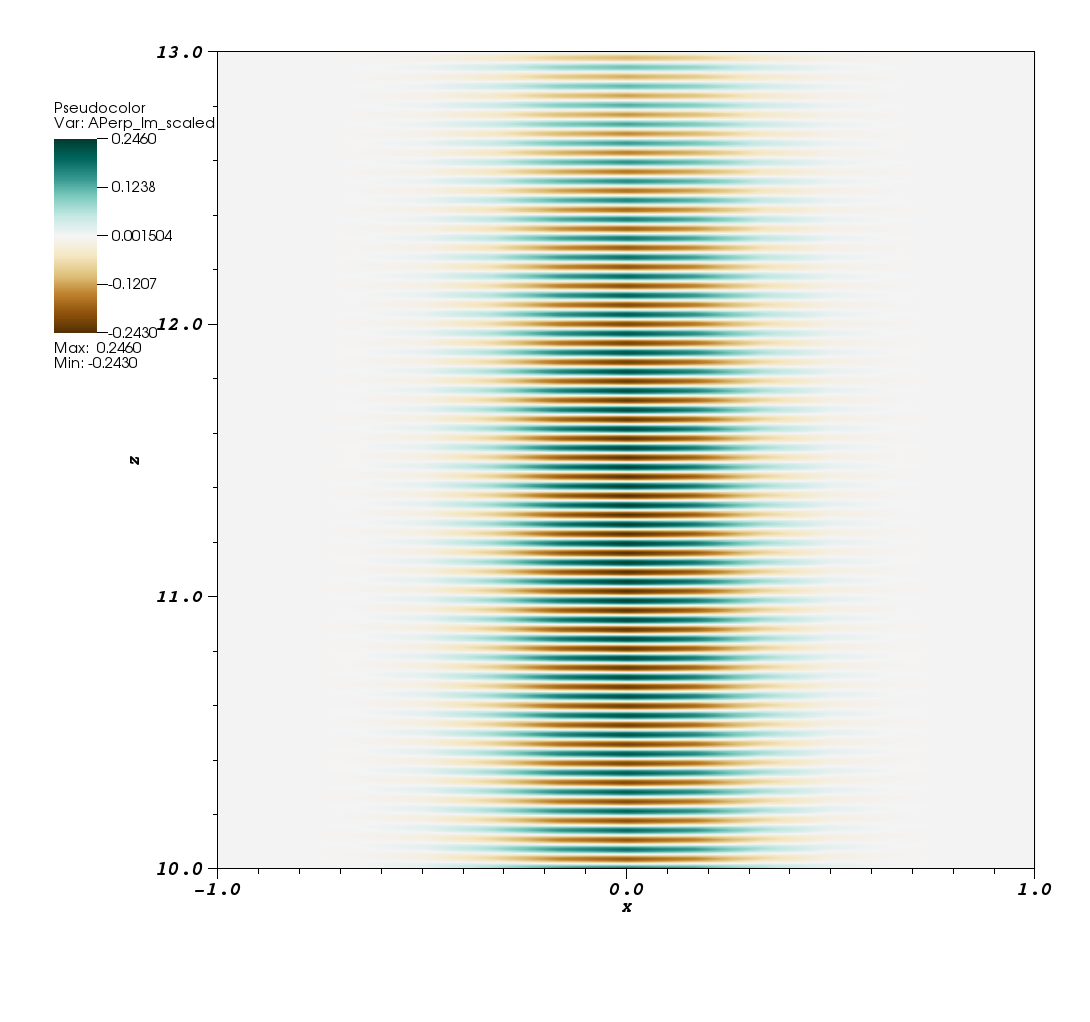
\includegraphics[width=100mm]{visit0036.png}
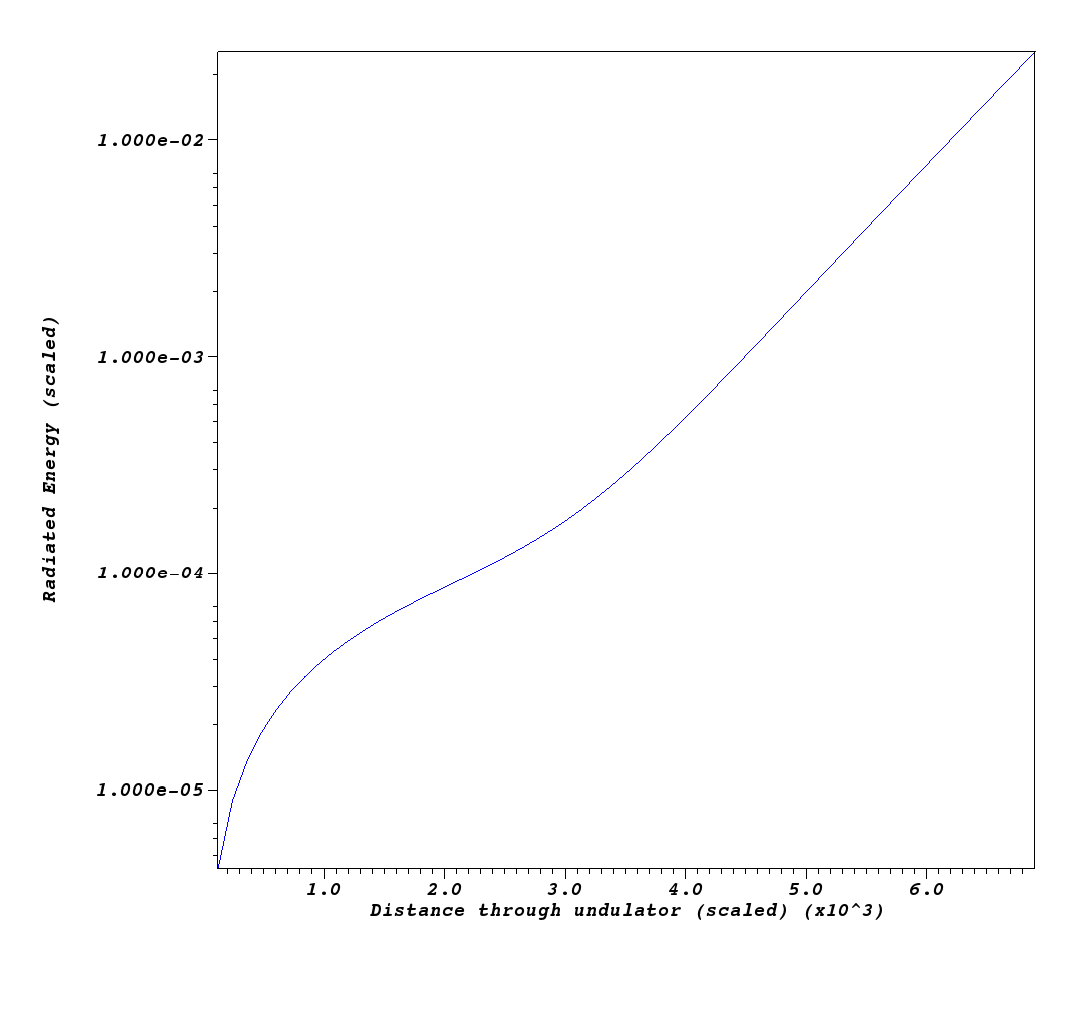
\includegraphics[width=100mm]{visit0037.png}
\caption{Radiated field from Puffin after amplification in the undulator - x polarized field (top). Radiated energy vs scaled distance through the undulator is on the bottom. Observe the noise from the previous figure has disappeared; the amplification process cause the electrons to align and radiate in phase.  }
\label{bbd2}
\end{figure*}

\newpage

\section{Overview}

Puffin, being an unaveraged FEL code, is quite distinct from other FEL codes in it's lack of restrictions on the radiation and electron bandwidth being modelled. Due to the nature of the code, and the likely use cases for such a code, we have attempted to create a resource which is a flexible tool for numerical scientific research into some more esoteric FEL physics and regimes, while still containing enough `realistic'  components to enable modelling of a current or future facility.

The main Puffin algorithm solves the FEL system in a scaled reference frame - see section \ref{puff-eqns} for a description. Data I/O may be in either SI or the Puffin scaled variables.

\subsection{Input Files}

At a minimum, one must specify 2 files for use in Puffin - a main input file, and a beam input file. The main file sets up the system scaling, the field mesh, the integration step sizes, and other simulation options. A simple, single undulator system can be setup here. It also specifies the names of the other input files, including the beam file.

The beam file specifies the electron beam parameters - there are 3 different types of beam input, detailed later in section \ref{beamfls}. Multiple beams can be specified, each with different characteristics, such as energies, lengths, charges, current profiles, etc.

Optionally, one may also supply a radiation seed file, to describe an injected radiation seed into the FEL with the electron beam. Similarly to the beam file, many radiation seeds can be specified here, at different frequencies, intensity profiles, \textit{etc}.

In addition, one may also supply a lattice file, which describes the layout of undulator modules, focusing quadrupoles, chicanes, drifts \textit{etc}. If this is not supplied, then a single undulator is set up as detailed in the main input file. If it is supplied, the wiggler in the main input file is ignored. Undulators can have independently variable polarizations, magnetic field strengths, etc. A description of available 3D undulator types is available in section \ref{und-fields}.

The main input file sets the frequency of data dumps from Puffin. Additionally, a `write file' can be supplied to give more flexibility and specify exactly when the data is written.

Puffin can be resumed from a previous run - if your cluster crashes, for instance. You could even resume from a previous run to extend or change undulator parameters, for instance.

Figure \ref{inputs1} shows a schematic of the Puffin input decks. Puffin comes with a few example input decks for reference.

\begin{figure*}
\centering
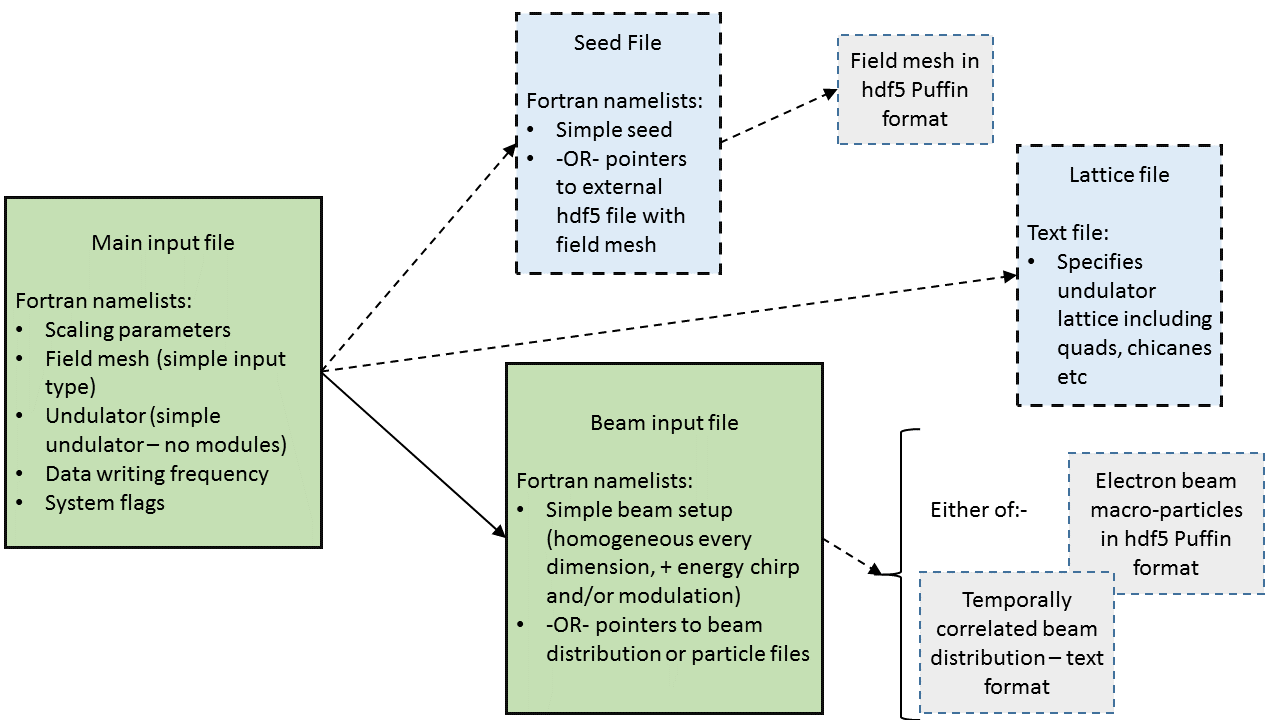
\includegraphics[width=120mm]{InputFiles.png}
\caption{Schematic of input files - dashed lines indicate optional files.}
\label{inputs1}
\end{figure*}



\subsection{To scale or not to scale?}

Although the Puffin algorithm uses scaled variables, the beam and radiation field parameters may be input in either SI units or the scaled units. Use the variable {\bf qscaled} in the main input file to specify whether scaled or SI units are being used. If $=$ {\bf .true.}, then Puffin expects scaled variables are being used. % If SI units are used, then the input parameters will be scaled according automatically to the scaling values specified in the main input file.

The main algorithm in Puffin utilizes the scaled variables above to make the numbers `nicer' to work with. The system saturates with scaled intensity $\sim 1$, the scaled perpindicular momentum of the beam in the wiggler oscillates between $-1$ and $1$, and so forth. The distance through the wiggler is given in units of a (1D) gain length, and the beam coordinate in the radiation frame is in units of the cooperation length, so that a reference electron slips $1l_c$ through the radiation field in $1$ gain  length. The scaling defines a frame of reference which normalises the quantities not only to numerically more manageable numbers, but to \textit{characteristic} variables.

The two dominant variables for the scaling are $\rho$ and $\eta$. $\eta$ is a function of the wiggler parameters $a_u$ and $\lambda_u$, and reference beam energy $\gamma_r$, and is calculated in Puffin from the input values of these 3 variables. It defines the velocity of the `reference' electron in the scaled radiation frame. The $\bar{z}_2$ coordinate is in the scaled frame travelling with the field (at velocity $c$) - $\eta$ determines how quickly the electrons slip back through this frame, such that an electron with energy $\gamma_r$, travelling in a wiggler with parameters $a_u$ and $\lambda_u$, slips back with scaled velocity $p_2 \equiv \dfrac{d \bar{z}_2}{d\bar{z}} = 1$.

The $\rho$ parameter is dependent on the peak electron beam number density, amongst other things, and as far as the discussion of the scaling parameters in Puffin goes, defines a reference for the amplification characteristics. A beam, or indeed, sections of an electron beam with peak number density giving a smaller `localised' $\rho$ will amplify the beam more slowly with respect to the reference beam specified by $\rho$.

That is to say, that they are only \textit{scaling} parameters. The FEL parameter as input by the user does not have to correspond to the beam or wiggler being input for the results to be correct. The scaled parameters will behave `nicely' if it does, but it is not necessary for the result to be physically correct. When the result is unscaled, the result will still be correct. The user may input in SI units, and get output in SI units. If using scaled units as input, the user must scale the lengths appropriately, but still, no beam input needs to satisfy the conditions to actually give the $\rho$ input by the user.






\begin{table}
\centering
\caption[Input Units]{Input Dimensions and Units for Beam and Radiation Field}
\begin{tabular}{|  c   | c  |   c   |}
\hline
Unscaled & units & unscaled equivalent (dimensionless) \\
\hline
$x$ & metres (m) & $\bar{x}$ \\
\hline
$y$ & metres (m) & $\bar{y}$ \\
\hline
$dx/dz$ & dimensionless & $\bar{p}_x$ \\
\hline
$dy/dz$ & dimensionless & $\bar{p}_y$ \\
\hline
$t$ & seconds (s) & $\bar{z}_2$ \\
\hline
\end{tabular}
\label{table}
\vspace*{-\baselineskip}
\end{table}



\subsection{3D Magnetic Fields}

\label{und-fields}

\subsubsection{Main Undulator Models}

The undulator is modelled analytically, and the model must include the fast wiggle motion. Puffin may be modified in the future to allow a map of the undulator field to be input. For now, there are a few generic undulator models employed. The undulator magnetic fields are chosen with the {\bf zundType} string in the main input file.

Available options for use in Puffin are `helical', `planepole' - corresponding to a planar wiggler with flat pole faces with natural focusing only in one direction, `curved' - correspnding to a planar undulator with curved, or canted, pole faces providing natural focusing in both transverse directions equally, and the default Puffin undulator, chosen with a blank string (`'), where the transverse polarization is chosen with the {\bf sux, suy} inputs, controlling the relative magnitudes of the peak magnetic fields in $x$ and $y$, respectively. These may vary between $0$ and $1$, allowing a general elliptic field to be described.

All of the undulator fields have an associated `natural' focusing channel, which arises from from the off-axis variation in the magnetic fields. This motion arises naturally when numerically solving the equations, and is not super-imposed artificially upon the electron motion.

\subsubsection{Undulator Ends}

The undulators also include entry and exit tapers, and they may be switched on or off in the input file with the flag {\bf qUndEnds}. Setting this to true will model a smooth taper up and down of the undulator magnetic fields in the first and last 2 periods of the undulator, taking the form of a $\cos^2$. If they are switched off, the beam is artificially initialized with an `expected' initial condition in the transverse coordinates for that undulator. Including these ends will model a more realistic and natural entry and exit from the undulator, and will reduce CSE effects from the shape of the wiggler.



\subsubsection{Natural Undulator Focusing}

Each undulator type has an associated natural focusing wavenumber. In the helical case, the natural betatron wavenumber is
\begin{align}
\bar{k}_{\beta n x} = \bar{k}_{\beta n y} = \frac{a_w}{2 \sqrt{2} \rho \gamma_0},
\end{align}
with $\gamma_0$ being the average energy of the electron beam (and not necessarily = $\gamma_r$, which only sets the scaling of the system.)

In the planar case,
\begin{align}
\bar{k}_{\beta n y} = 0, \\
\bar{k}_{\beta n y} = \frac{a_w}{2 \sqrt{2} \rho \gamma_0}.
\end{align}

In the canted pole case,
\begin{align}
\bar{k}_{\beta n x,y} = \frac{a_w \bar{k}_{x,y}}{\sqrt{2 \eta} \gamma_0},
\end{align}
where $\bar{k}_{x,y}$ describe the hyperbolic variation in the transverse directions (see eqns (\ref{cp1} - \ref{cp3})), and must obey
\begin{align}
\bar{k}_x^2 + \bar{k}_y^2 = \frac{\eta}{4 \rho^2}
\end{align}
to be physically valid. They determine the focusing strength in the $\bar{x}$ and $\bar{y}$ dimensions. For the case of equal focusing, then,
\begin{align}
\bar{k}_{\beta n x} = \bar{k}_{\beta n y} = \frac{a_w }{ 4 \rho \gamma_0}.
\end{align}



\subsubsection{Strong Beam Focusing}

In addition to the natural focusing channel, a constant, `strong' focussing channel may be utilized, to focus the beam to a smaller transverse area. This is a magnetic field super-imposed upon the wiggler. It may be switched on or off with the flag {\bf qFocussing} in the main input file, and is specified through the use of the variables {\bf sKBetaXSF} and {\bf sKBetaYSF}. It is probably highly artificial - it may be thought of as physically similar to an ion channel. Nevertheless it allows one to obtain strong focusing without using a lattice. It is defined very simply as
\begin{align}
b_x = \sqrt{\eta} \frac{\bar{k}_{\beta y}^2}{\kappa}\bar{y}_j, \\
b_y = - \sqrt{\eta} \frac{\bar{k}_{\beta x}^2}{\kappa}\bar{x}_j
\end{align}

If either {\bf sKBetaXSF} or {\bf sKBetaYSF} are not specified, then no focusing channel will be added for that dimension, even if the {\bf qFocussing} flag is true.

Magnetic quads between modules can be specified in the lattice file. See section \ref{latt-file}.


\subsubsection{Auto beam-matching}

The beam, when specified by the `simple' method (see below) may be matched to the focusing channel of the undulator automatically with the flag {\bf qMatched\_A} in the beam file - the option can be set for each beam. (Note this is for the natural or enhanced \textit{undulator} focusing, and matching is not performed for a FODO lattice!) In the scaled notation,
\begin{align}
\bar{\sigma}_{x,y} = \sqrt{  \frac{ \rho \bar{\epsilon}_{x,y} }{\bar{k}_{\beta x,y} }  }
\end{align}
where $\bar{\epsilon}_{x,y} = \epsilon_{x,y} / (\lambda_r / 4\pi)$ are the transverse emittances scaled to the so-called Kim criterion.

%If we define $\bar{a}_w$ as the $rms$ undulator parameter, so that  $\bar{a}_w = a_w$ in the helical case, and  $\bar{a}_w = a_w / sqrt{2}$ in the planar and canted pole case, then we can write a general expression


The spread in the transverse momentum directions is then given by
\begin{align}
\bar{\sigma}_{px, py} = \frac{\sqrt{\eta}}{2 \kappa} \Bigl<  \frac{\Gamma}{1+\eta p_{2}}  \Bigr> \frac{ \bar{\epsilon}_{x,y} }{\bar{ \sigma}_{x,y}}.   \label{tmtch_spd}
\end{align}
where angular brackets indicate the ensemble average of the beam.

If {\bf qFocussing} is true and the strong betatron wavenumber is given, then the strong betatron wavenumber is used to match the beam. Otherwise the beam is auto-matched to the natural focusing channel of the undulator. As this matching is done only for the in-undulator focusing, and not for the FODO lattice, the Twiss ($\alpha_x, \alpha_y$) input parameters will be ignored if {\bf qMatched\_A = .true.} in the input. If one wishes to use a FODO lattice, the matching must be done by the user - the matched Twiss parameters are not calculated by Puffin. See section \ref{section-twiss} for how to input Twiss parameters.



\subsubsection{Twiss Parameters}

\label{section-twiss}

One can use Twiss parameters to provide a transverse phase-space `tilt' for the electron beam. In the simple beam case, the user can specify the \textit{r.m.s.} $\bar{\sigma}_x, \bar{\sigma}_{px}$ (or the S.I. equivalents $\sigma_x, \sigma_{x}'$) for the electron beam, along with the usual $\alpha_x$ for the slope of the $x-x'$ correlation. Using this method, the supplied \textit{r.m.s.} $\sigma_{x}'$ should be the standard deviation at $x=0$. If the emittance is supplied by using {\bf emitx}, then the input $\bar{\sigma}_{px}$ is ignored, and is instead calculated from $\sigma_x$, the emittance, and $\alpha_x$. Obviously, the intended method is to input the emittances, so that the transverse momenta parameters are over-written.

% In general, giving the emittances over-writes the transverse momenta given in the beam file, whether using the




%%% Beam energy - what is the unscaled input?
%%% Have to explain the 'mean' beam energy and
%%% the rms width in energy are in what units...??










\subsection{Beam Initialization}
\label{beamfls}
There are 3 different ways of defining and initializing the electron beam in Puffin:

\subsubsection{Simple}

The beam is described in terms of a homogeneous Gaussian function in every dimension. Some simple correlations in energy can be achieved by specifying an oscillation in the beam energy as a function of $\bar{z}_2$, or as a simple linear energy chirp in $\bar{z}_2$. Twiss parameters may be used to tilt the beam for matching to a FODO lattice (Puffin does not calculate the matched Twiss parameters - this must be done separate to Puffin). The beam is generated in Puffin according to this description.

In general, the correct noise statistics are added to the beam with the method described in \cite{noise1}. This method, like other beam noise algorithms for FELs, requires a quiet beam to add the noise to. We include two methods of generating the beam - one with the correct noise in all dimensions, and one with the correct noise only in the temporal/$\bar{z}_2$ dimension. In both methods, the beam is initially quiet in the temporal dimension before adding the noise, with an equispaced layout of the particles in this dimension. The beam MUST be created to appropriately sample the wavelength of emission/amplification - so at least 10 equispaced particles per resonant wavelength. The methods are:-

% qSI - input in SI units - so x, y, z, px, py and gamma - system is then scaled to rho
% Rho and charge are decoupled - so the simulation will always be correct. For the scaled notation to make sense, the rho must be approximately correct for the given beam charge.
% qEqui = .false. by default.



{\bf Equispaced Grid in Every Dimension}

When using this option, the beam is intialized on an equispaced 6D grid. This requires very many particles to appropriately sample every dimension, and you may find it very easy to have more macroparticles than real electrons while loading the beam this way. However, we leave it up to the user to decide if this is appropriate - for some extreme dispersion situation with high charge it may be necessary to create the beam in this way.  This can be activated by setting {\bf qEquiXY $=$ .true.} in the beam input. {\bf qEquiXY} is actually an array of size nbeams, with a seperate value for each beam if multiple beams are desired. {\bf qEquiXY $=$ .false.} by default.

{\bf Equispaced grid ONLY in $\bar{z}_2$}

If qEquiXY is false, then the beam is intially generated as a 1D beam, with equispaced macroparticles. Each macroparticle is then split into many particles in the other 5 dimensions, with coordinates generated by a quasi-random sequence in each dimension. The SAME SEQUENCE is used for each particle in z2 - the creates a series of beamlets in the $\bar{z}_2$ dimension, giving a quiet start in $\bar{z}_2$. Because random sequences are used, the other 5-dimensions require orders of magnitude less particles to adequately fill the phase space than in the equispaced case. This is the default option, so if not specified, {\bf qEquiXY $=$ .false.}.

Both of the above methods may, of course, be replicated and modified by the user to suit a particular situation. The creation of the beam with the correct statistics, while still retaining the sampling necessary for the FEL interaction, is still an area of ongoing research, and is quite controversial, especially when including large velocity disperion in the beam dynamics. We ultimately leave it to the user to ensure the beam is appropriately initialized for their situation. The methods above can probably be replicated with just a few lines of \textit{e.g.} Python. The generated beam can then be input into Puffin.

To use this, set the option dtype = `simple' in the nblist namelist in the beam file. The parameters for the distribution are then set in the blist namelist in the same file.

\subsubsection{Dist input}

The input is composed of a description of temporal slices along the bunch, describing a Gaussian mean and standard deviation in every other dimension, along with Twiss $\alpha$ parameter, for each temporal slice. This information is used to generate the electron beam in Puffin. The slices must be spaced finely enough to sample the radiation field wavelength being amplified - so \textit{e.g} at least 10 per wavelength.

\subsubsection{Beam input}

This method allows one to read in the 6D scaled particle coordinates from an HDF5 file or a text file. The HDF5 file should be in the same format as the Puffin output. The text input is not recommended, especially for 3D runs, since the reading in is very inefficient, and the files are usually huge for 3D data. The beam is generated externally, and the user is then responsible for ensuring the sampling and the noise in the pulse are correct - it is not added by Puffin in this method.


\subsection{Field Mesh}


The radiation field in Puffin is modelled by a simple cartesian mesh, with equispaced nodes in each of the 3 spatial dimensions. Each node samples a value of the $x$ and $y$ polarized radiation field (the $z$ component of the electric field is not modelled). The scaled $\bar{z}_2$ coordinate frame is such that the back of the system is with increasing $\bar{z}_2$ - \textit{i.e.} to the right in figure \ref{lgmsh}. Recall that $\bar{z}_2$ is the stationary radiation frame, so that as the beam propagates through the undulator, the beam slips back through the radiation field, moving to the right in figure \ref{lgmsh}.

This mesh must be large enough to contain the beam through the entire propagation distance through the wiggler.

It must also be large enough to contain the beam in the transverse plane, see figure \ref{trmsh}. The radiation field is calculated from the driving electron beam by linear interpolants, so the field must adequately sample the area which the beam occupies.  The radiation also diffracts outwards from the beam, so the field mesh must extend to adequately model this diffracting radiation to avoid numerical problems at the boundaries of the grid. There are absorbing boundaries in the outer 16 nodes in the mesh in $x$ and $y$ to mitigate this issue, but an absorbing boundary which works well for the full range of frequencies modelled by Puffin is difficult to realise, and the absorbing boundary should not be relied upon to absorb everything which propagates to the outer reaches of the mesh.

\subsubsection{Fixing the Radiation Mesh}

One may use the variables {\bf iRedNodesX, iRedNodesY} to fix the mesh around the beam when initializing a simple beam - see figure \ref{trmsh}. These variables define an inner set (`reduced' set) of nodes which the beam width will occupy. So the mesh length in $x$ and $y$ will be set up such that the inner set of nodes defined by  {\bf iRedNodesX, iRedNodesY} will contain the beam. In this case, the {\bf sFModelLengthX, sFModelLengthY} inputs will be ignored.


\begin{figure*}
\centering
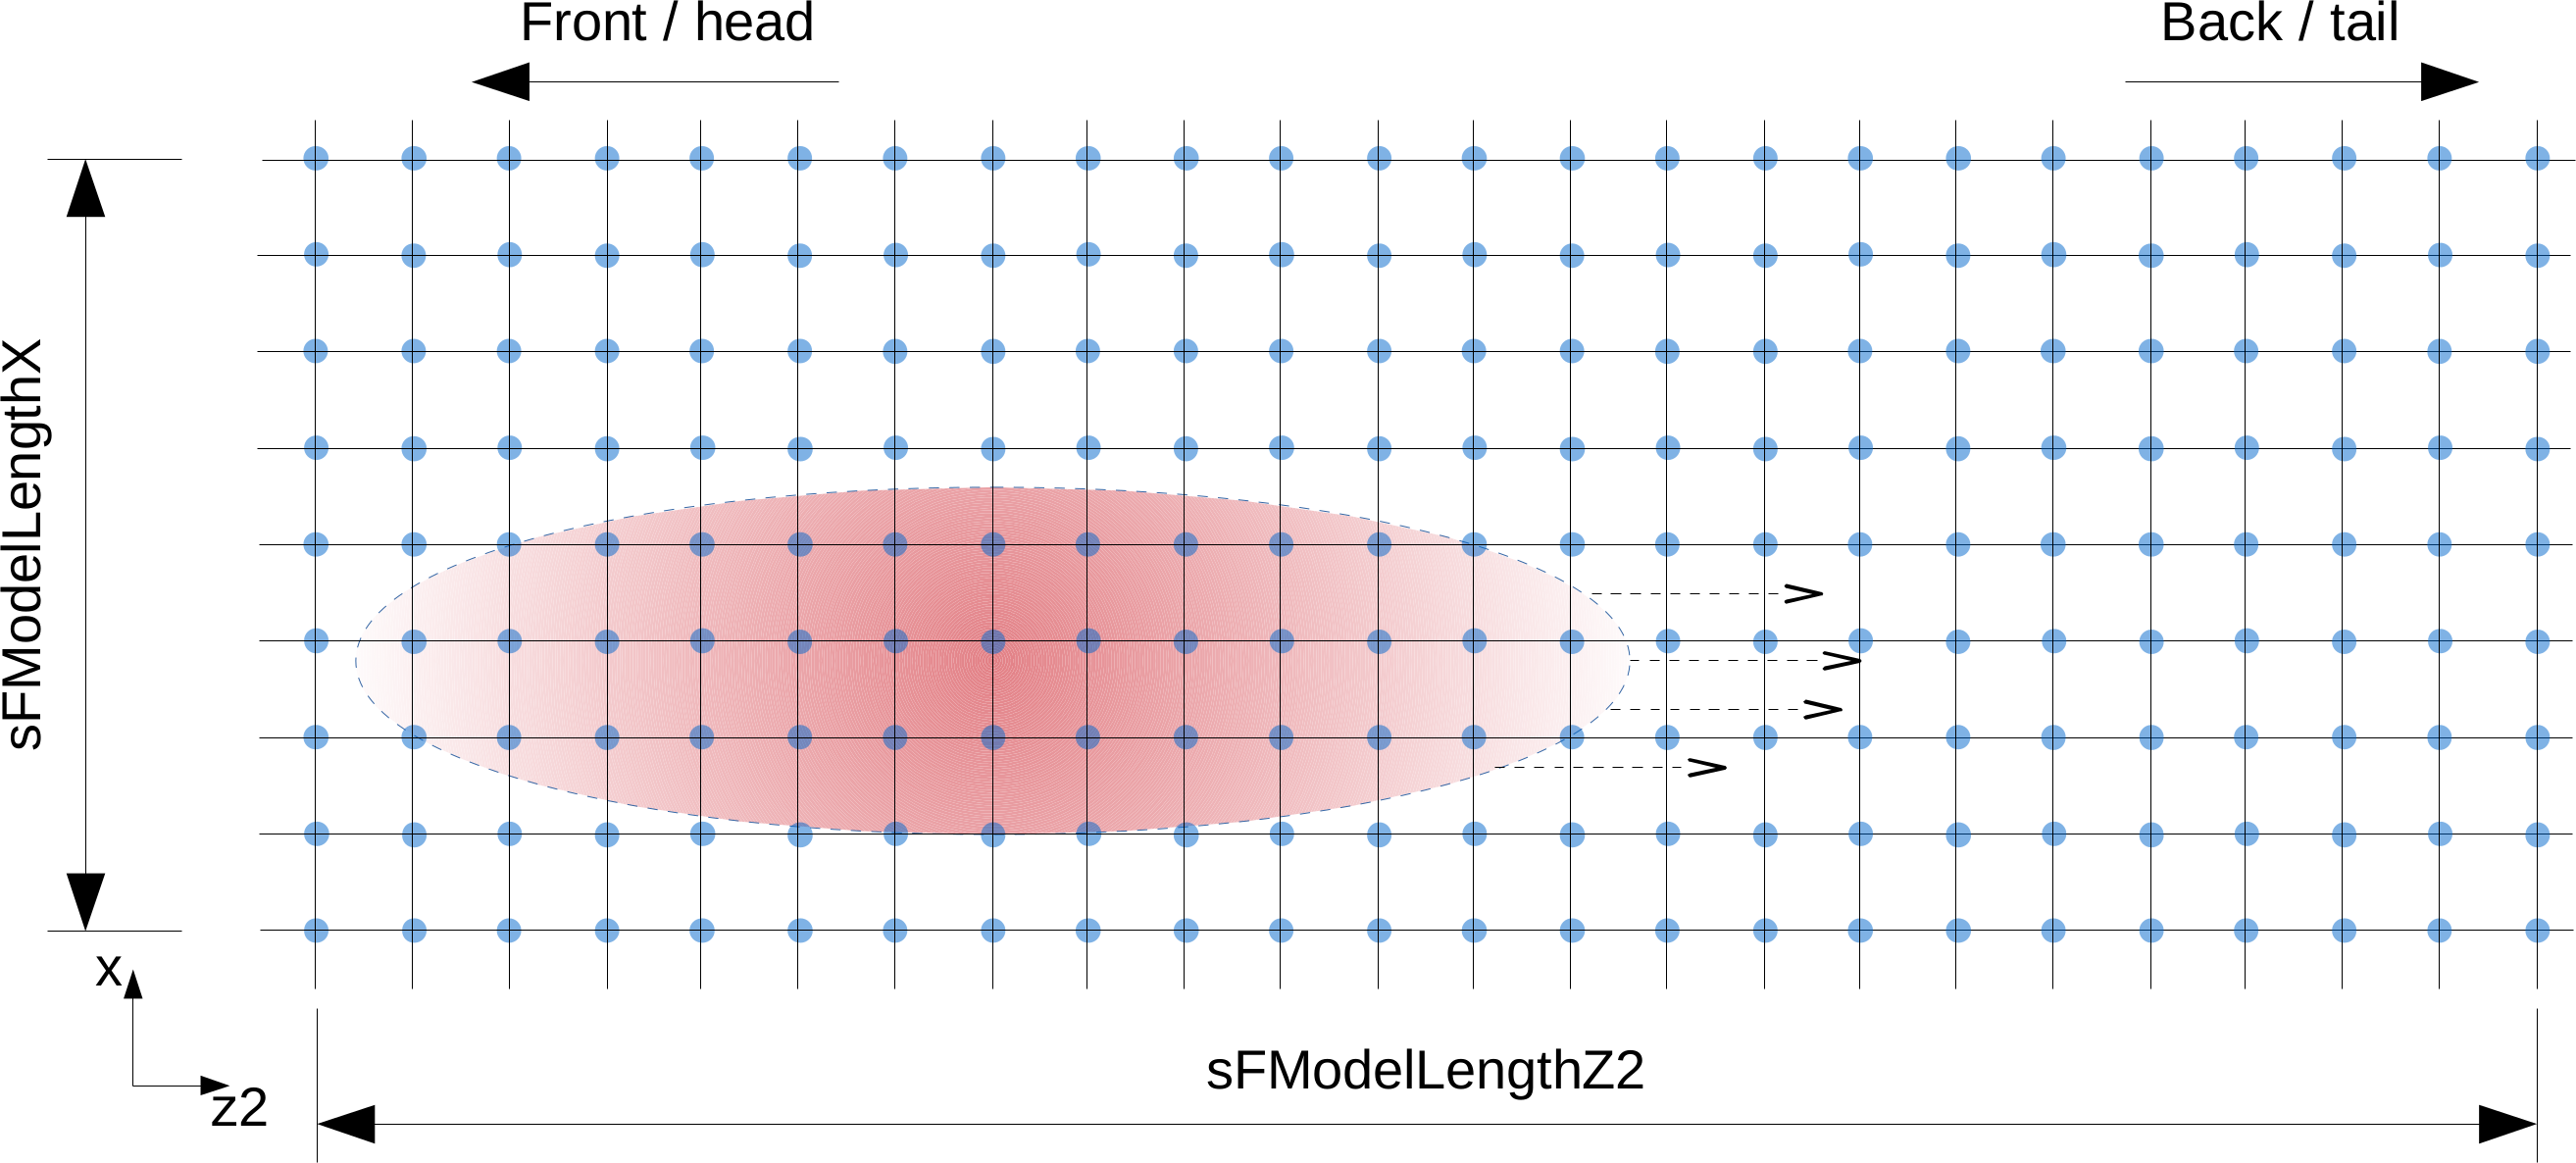
\includegraphics[width=150mm]{long_mesh.png}
\caption{Showing the longitudinal setup of the radiation mesh. The beam is indicated in red. The scaled $\bar{z}_2$ coordinate is defined so that the front of the radiation and beam is to the left. This is the constant radiatioon frame, so the beam slips backwards through the field from left to right. In the lab frame, the beam and radiation propagates from right to left. The full length of the mesh must be large enough to contain the beam through propagation.}
\label{lgmsh}
\end{figure*}


\begin{figure*}
\centering
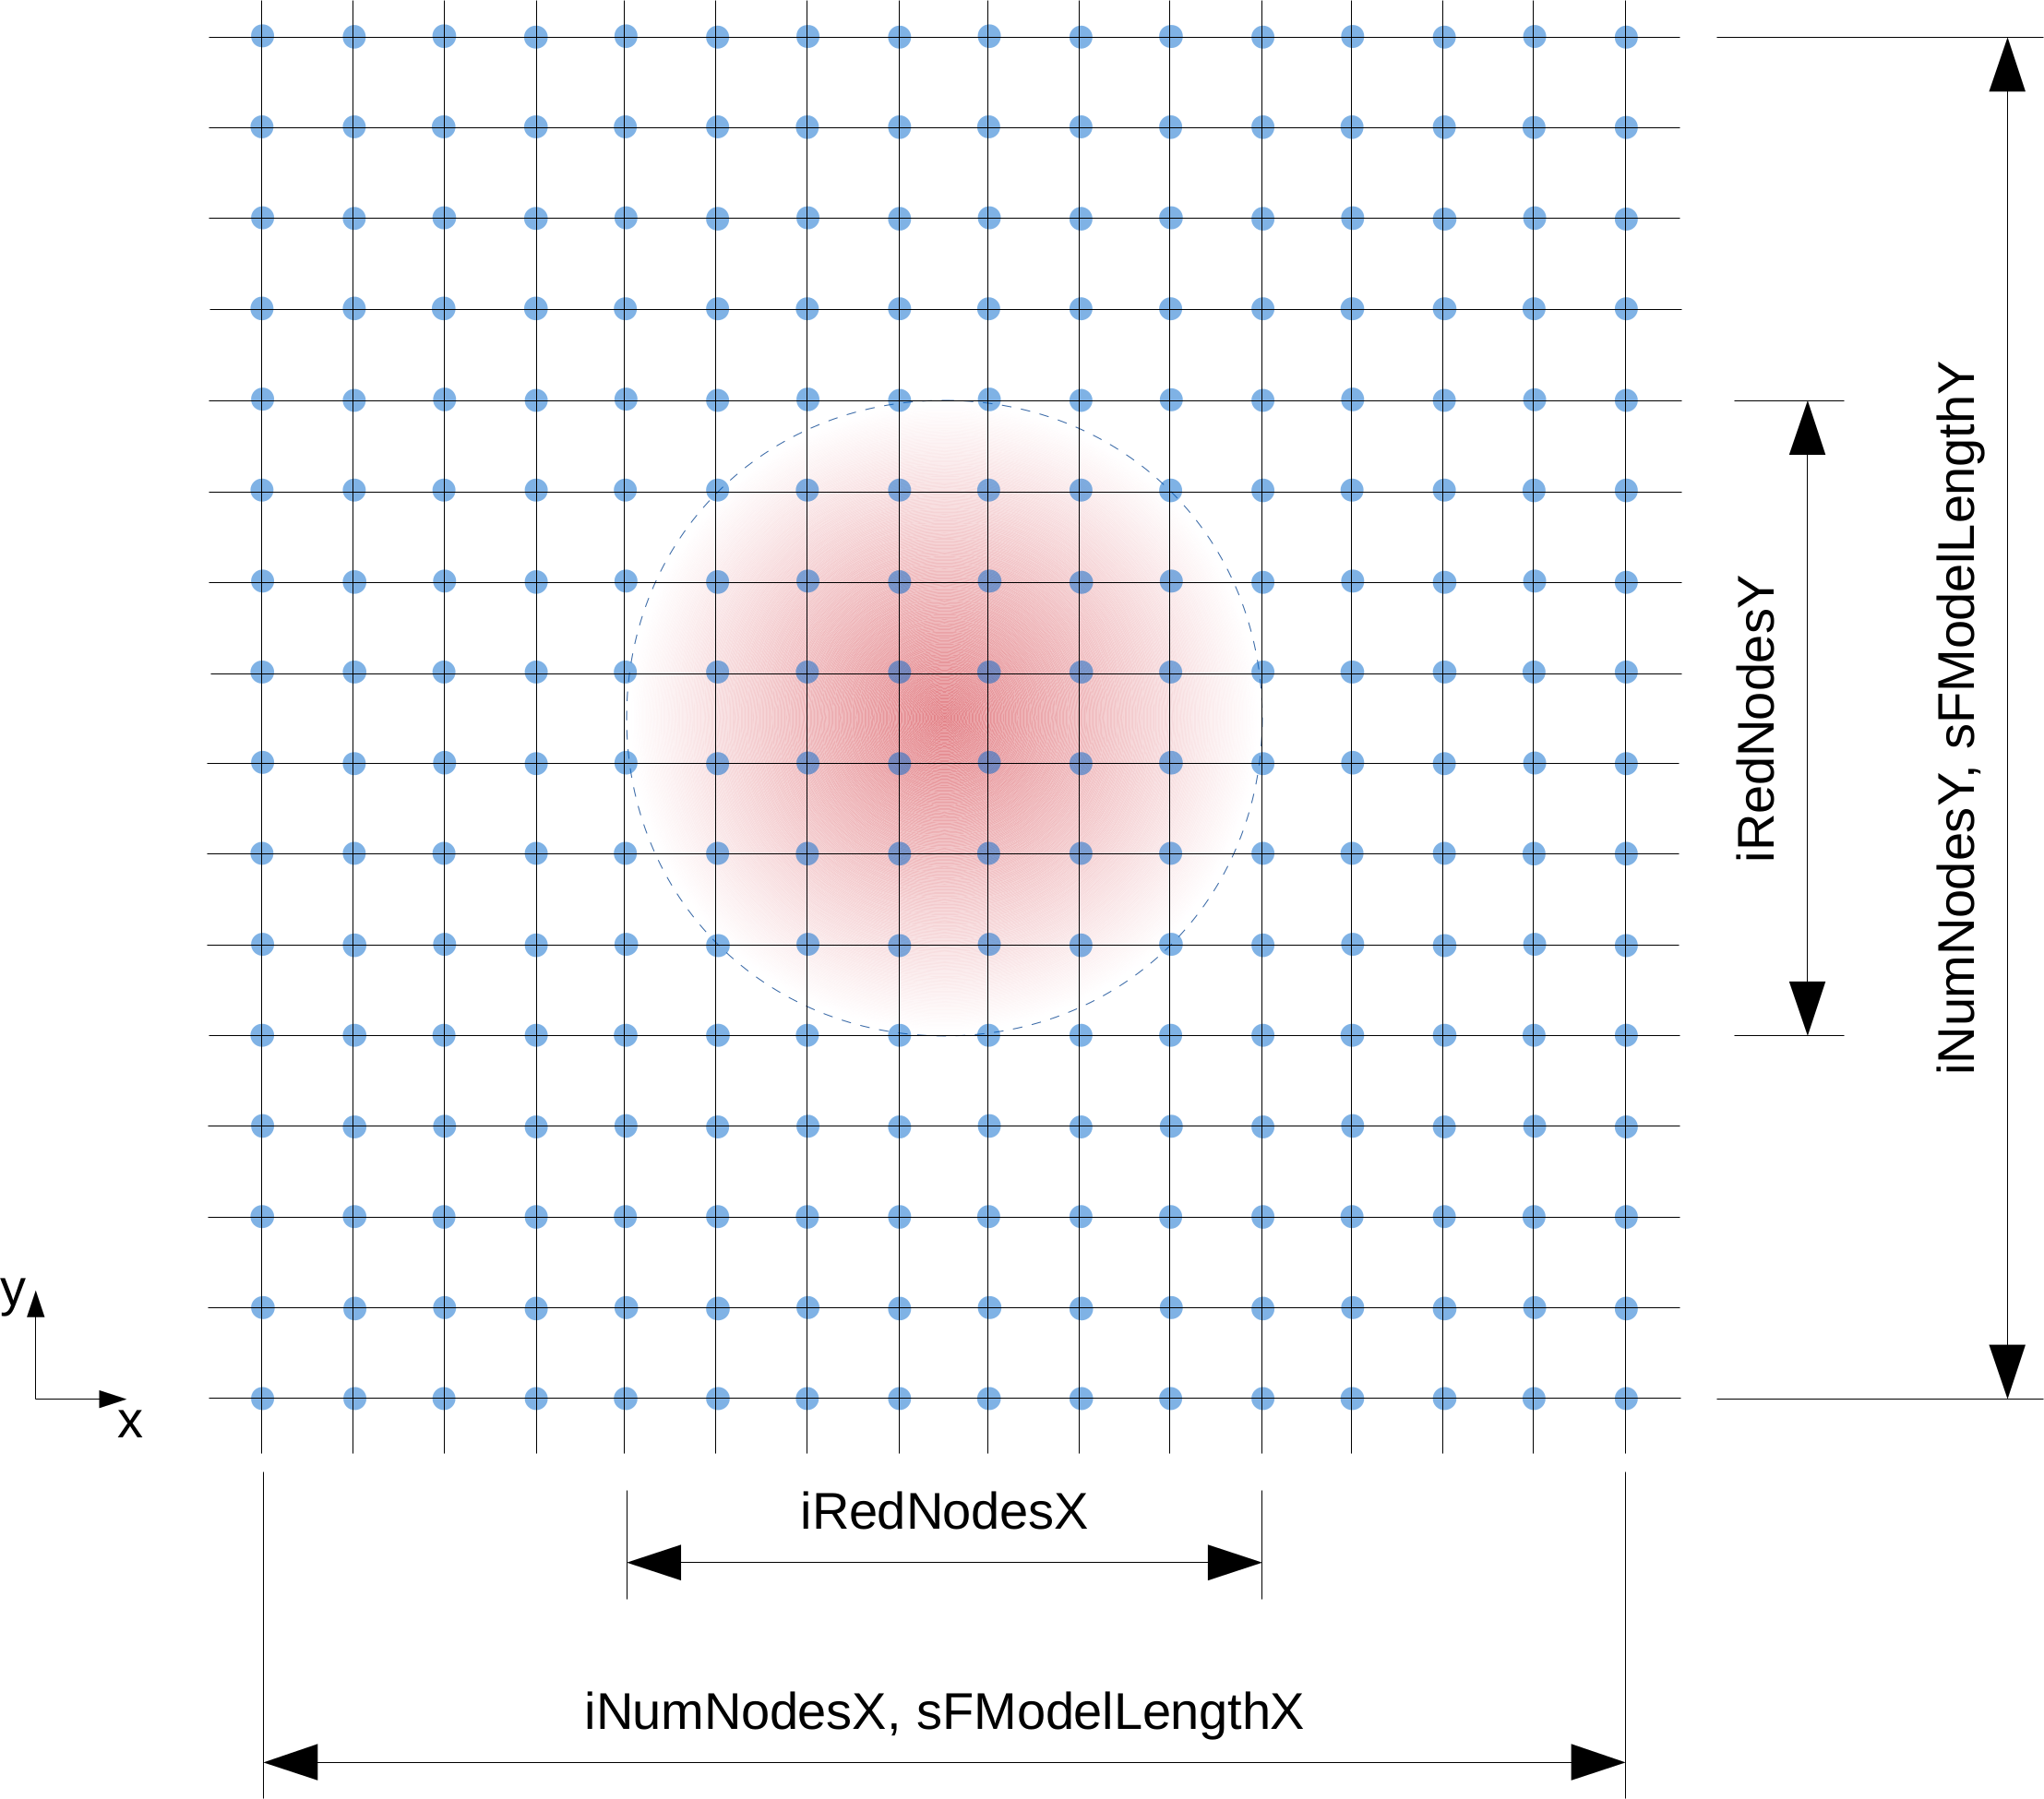
\includegraphics[width=150mm]{trans_mesh2.png}
\caption{Transverse mesh to model the radiation field - the beam is indicated in red. The mesh may be `matched' to the transverse beam profile initially by specifying the iRedNodes parameters - these specify an inner set of nodes such that the mesh will be setup so that the beam is contained within this number of nodes (when using the simple beam input type only). This is only an initial condition, but can aid in setting up the mesh.}
\label{trmsh}
\end{figure*}



\subsection{Lattice Input}

\label{latt-file}

A lattice file may be supplied in the main input file with the variable `lattFile'. This is the name of the lattice file, containing details of the undulator module lattice layout. If blank, then a single undulator as specified in the main input file will be used.

The lattice file is a plain text file, where each line beginning with one of the two-letter identifiers below, and in table \ref{tableLat}, represents a lattice element. There are five supported lattice element types, being undulators, quads, chicanes, drifts, and modulations. These are specified in the lattice file by the first 2 characters of each line, followed by (on the same line) the options for the element. Any line not beginning with one of these identifiers is ignored.


\begin{table}
\centering
\caption[Input in Lattice File]{Accelerator components for use in lattice file}
\begin{tabular}{|  c   | c  |}
\hline
Component & ID Initials  \\
\hline
Undulator & {\bf UN} \\
\hline
Quadrupole & {\bf QU} \\
\hline
Chicane & {\bf CH} \\
\hline
Drift & {\bf DR} \\
\hline
Modulation & {\bf MO} \\
\hline
\end{tabular}
\label{tableLat}
\vspace*{-\baselineskip}
\end{table}




%Undulator - UN

%Quadrupole - QU

%Chicane - CH

%Drift - DR

%Modulation - MO

Each entry must be followed by the options specifying that lattice element, on the same line, delimited by spaces.

{\bf UN} - Undulator Module

For the undulator,  one must specify the undulator type, the number of wiggler periods $N_w$, the undulator parameter relative to the base undulator parameter in the main input file $\alpha$, the linear taper $\dfrac{d \alpha}{d \bar{z}}$, the polarization $u_x$ and $u_y$ (ignored for the non-variable polarized undulator types), a logical specifying if undulator ends are being used for this module, another logical spcifying if a strong focusing channel is being used in the undulator, and the strong focusing strengths $\bar{k}_{\beta x}$ and $\bar{k}_{\beta y}$, and the number of integration steps per period to be used in this module.

{\bf QU} - Quadrupole

For the quad, we must specify $\bar{F}_x$ and $\bar{F}_y$. These are scaled transverse components of the transform matrix for the quad. The quad is only a point transform, currently, and does not have a length, so the length must be included in a drift section. The transforms for the quad, in S.I. units, are defined as
\begin{align}
\frac{d x_j}{d z}  \bigg|_{new} = \frac{d x_j}{d z} \bigg|_{old} + \frac{1}{F_x} x_j \\
\frac{d y_j}{d z}  \bigg|_{new} = \frac{d y_j}{d z} \bigg|_{old} + \frac{1}{F_y} y_j
\end{align}
which in the scaled notation becomes:
\begin{align}
\frac{d \bar{p}_{xj}}{d \bar{z}} \bigg|_{new} = \frac{d \bar{p}_{xj}}{d \bar{z}}  \bigg|_{old} +\frac{\sqrt{\eta}}{2\rho\kappa} \frac{\bar{x}_j}{\bar{F}_x} \\
\frac{d \bar{p}_{yj}}{d \bar{z}}  \bigg|_{new} = \frac{d \bar{p}_{yj}}{d \bar{z}}  \bigg|_{old} +\frac{\sqrt{\eta}}{2\rho\kappa} \frac{\bar{y}_j}{\bar{F}_y}
\end{align}
where $\bar{F}_{x,y} = \dfrac{F_{x,y}}{l_g}$.

In $x$ (unscaled) focal length is taken as
\begin{align}
\frac{1}{F_x} = \frac{g L_Q}{B\rho},
\end{align}
where $g$ is the quad magnetic field gradient in $Tm^{-1}$, $L_Q$ is the length of the quad, and $B\rho = \beta E_0 / 0.2998$ is the so-called magnetic rigidity in $Tm$, with the beam energy $E_0$ in $GeV$ (corresponding to the scaling energy defined in the input file).

{\bf CH} - Chicane

For the chicane, one must specify physical length, slippage length, and dispersion enhancement (scaled R56). The length is the physical length of the device in undulator periods, and is used to calculate the diffraction properly. The slippage length tells how many wavelengths to delay the beam by relative to the radiation field in resonant radiation wavelengths - be careful, this should not be $\leq 0$, or the beam will then be faster than light speed! Similarly, it is left up to the user to decide what is appropriate to delay the beam by with respect to the physical length of the device. The dispersive enhancement, $D$, is the scaled R56 of the device - using $\gamma_r$ in the main input as the mean $\gamma$ for the chicane, so that
\begin{align}
\bar{z}_{2} = \bar{z}_{20} - 2D \left( \frac{\gamma - \gamma_r}{\gamma_r}  \right),
\end{align}
and $D = k_r \rho  R_{56}$.

This approach of being able to vary the 3 parameters above is quite flexible, but at the expense of easy automatic checking of the physical relevance of the parameters. For example, one can disperse the beam 'in place', without shifting it w.r.t. the resonant wavelength, which is obviously unphysical. However, this may be useful for a quick setup of the beam for EEHG at the beginning of the undulator, for instance. If one is not sure of the physical length of the actual device, but knows the length between modules and the desired slippage (e.g. for mode locking the FEL), then one can specify the spatial drift between modules using a drift section, and then specify a chicane with zero physical length, but with the desired delay and R56. In this way the radiation diffraction will still be modelled correctly.

{\bf DR} - Drift

For the drift, one must specify length in units of the number of undulator periods.

{\bf MO} - Modulation

For the modulation section, one may add an energy modulation to the beam specified by $\bar{k}_M = \dfrac{2 \pi}{\bar{\lambda}_M}$ and $\dfrac{\Delta \gamma}{\gamma_r}$.


\newpage

\section{Numerical Model}

\newpage

\section{Data Output and Post-Processing}

\subsection{Data Output}

Data output is classified as either `full' or `integrated' (reduced) data. The full data dumps consist of the $x$ and $y$ field values on the field mesh, and the macroparticle coordinates in 6D phase space. In a 3D run, this data can easily be $>100$GB's per dump, so it is advisable to limit the frequency of the dumps, which is controlled in the main input file by the variable {\bf iWriteNthSteps}.

On the other hand, the reduced data sizes are much smaller, and typically can be written every undulator period. It can still be quite large, depending on the modelled FEL and length of the run, but it will always be significantly smaller than the full data dumps for 3D runs. Integrated data includes quantities like radiation power, bunching, energy spread, current, emittance, beam radius \textit{etc} as functions of $\bar{z}_2$ or $ct-z$. Frequency of the integrated dumps is controlled with {\bf iWriteIntNthSteps} in the main input file.

\subsection{Output Format}

When running Puffin, a few different files will be produced besides the data output files. A *.log file provides any information on errors. A rec.out file tracks the step number the simulation is at in the main integration loop (this is also printed to standard out, but on some job submission systems the stdout will not be visible till AFTER the job has finished. rec.out should be available as the job is running to track the job progress).

The data output is usually in the HDF5 file format, or optionally in the SDDS format. Currently, SDDS support is quite limited, and full data dumps and only the radiation power of the integrated data is output. Much more integrated data is output in the HDF5 files.

\subsubsection{HDF5}

The HDF5 file naming convention in Puffin is: $<$basename$>\_<$type$>\_<$step$>$.h5, where basename is the input file basename (i.e.the input file name without the postfix `.in')

Type can be integrated, aperp, or electrons, corresponding to reduced or integrated data, a full dump of the field mesh (x and y polarised fields), and a full dump of the electron macroparticle coordinates $+$ charge weight. These are described individually in more detail below. Due to the possible extremely large size of the full dumps, one should be careful how often the data is being written.

One may simply choose which steps to write out through use of the {\bf iWriteNthSteps} and {\bf iWriteIntNthSteps} parameters in the main input file. The former controls the frequency of the full dumps, and the latter specifies the frequency of the integrated data writes.

In addition, one may activate the {\bf qDumpEnd} flag to write a full dump at the end of the simulation - this is {\bf .true.} by defualt, but may be switched off.

More useful is the write file. This allows one to specify the exact step numbers at which to write out the full dumps. This will be done in addition to the regular write intervals specified above. The file is pointed to from the main input file by the string {\bf wr\_file}. In this plain text file, specify each step to write at with a line beginning with {\bf WR}, followed by a space (or multiple spaces) and then the step number. Any line not beginning with {\bf WR} will be ignored.

\subsection{Output Format Specification}

Puffin uses primarily hdf5 for output, although sdds dumps can be made if desired. The sdds outputs do not contain the integrated data, except power.

For input filename $=$ {\bf basename.in}, then outputs are as described:

\subsubsection{Full Dumps}

Two files for each step written out - one for the field mesh, and one for the macroparticle positions.

{\bf Field Mesh}

Named {\bf \textit{basename}\_aperp\_\textit{stepnum}.h5}, where {\bf stepnum} is the integration step number the data was written out at. The file has internal hdf5 structure:

\begin{lstlisting}[language=python, caption=Structure of HDF5 field output file produced by Puffin]
/ (RootGroup)
/aperp (Array(2, nz2, ny, nx))
/globalLimits (Group)
/intensityScaled (Group)
/meshScaled (Group)
/runInfo (Group)
/time (Group)
\end{lstlisting}

The {\bf aperp} dataset contains the values of the field at each field node. {\bf nz2}, {\bf ny} and {\bf nx} are the number of nodes in the equispaced field mesh in $\bar{z}_2$, $\bar{y}$, and $\bar{x}$, respectively. The data {\bf aperp(1,:,:,:)} contains the values of the x-polarized field, and {\bf aperp(2,:,:,:)} is the \textit{negative} y-polarized field.  It also contains some data about the run itself (some of this data is also in the runInfo group in the file). An example of the data is:-

\begin{lstlisting}[language=python]
    iChic_cr := 1,
    iCsteps := 0,
    iDrift_cr := 1,
    iL := 0,
    iModulation_cr := 1,
    iQuad_cr := 1,
    iUnd_cr := 1,
    istep := 0,
    numSpatialDims := 3,
    time := 0.0,
    vsAxisLabels := 'xbar,ybar,z2bar',
    vsCentering := 'nodal',
    vsIndexOrder := 'compMajorF',
    vsLabels := 'aperp_real, aperp_imaginary',
    vsLimits := 'globalLimits',
    vsMesh := 'meshScaled',
    vsNumSpatialDims := 3,
    vsTimeGroup := 'time',
    vsType := 'variable',
    zInter := 0.0,
    zLocal := 0.0,
    zTotal := 0.0,
    zbarInter := 0.0,
    zbarLocal := 0.0,
    zbarTotal := 0.0
\end{lstlisting}

The integers ending in `cr' are counters for the lattice elements which may be present - {\bf iChic} is for the chicane, {\bf iQuad} is for the quads, {\bf iUnd} is for the undulator modules, {\bf iModulation} is for the beam modulator sections, and {\bf iDrift} is for the drift sections. The counter number indicates that the beam has been been completely through the counter number $-1$ (so in the example shown, it has been through no components yet.)

{\bf istep} is the number of completed integration steps through the current undulator module. It is local to the module being integrated through when the data was written.

{\bf iCsteps} is the number of \textit{total} (cumulative) integration steps completed through the entire undulator line, including all previous undulators.

The {\bf zInter, zLocal} and {\bf zTotal} values are distances through the machine, in metres. {\bf Inter} indicates the \textit{interaction} distance through the machine - that is, the distance of undulators only, discounting the drifts, chicanes, etc. {\bf Local} is the distance through the local undulator module. {\bf Total} is the total distance through the machine when the data was written.

{\bf zbarInter, zbarLocal} and {\bf zbarTotal} correspond to {\bf zInter, zLocal} and {\bf zTotal}, scaled to $L_g$, the 1D gain length.


The {\bf intensityScaled} group is a VizSchema derived variable, which tells Visit how to calculate the intensity from the scaled field data.

The {\bf meshScaled}, {\bf globalLimits} and {\bf time} groups are VizSchema metadata for \textit{e.g.} Visit.

{\bf runInfo} is a group containing data about the run the data is from. It includes data about the physical parameters, the scaling and the mesh sizes, amongst other things. A listing of the metadata in this group is here:

\begin{lstlisting}[language=python]
    Lc := 1.5887624436132764e-06,
    Lg := 0.43767608132326558,
    aw := 1.0121808999999999,
    eta := 3.6299960436719031e-06,
    gamma_r := 456.39999999999998,
    iChic_cr := 1,
    iDrift_cr := 1,
    iModulation_cr := 1,
    iQuad_cr := 1,
    iUnd_cr := 1,
    kappa := 0.22177495617879053,
    lambda_r := 9.9824891200977331e-08,
    lambda_w := 0.0275,
    nSteps := 870,
    nX := 120,
    nY := 120,
    nZ2 := 161939,
    npk_bar := 302255429.89145231,
    rho := 0.0050000000000000001,
    sLengthOfElmX := 0.033613445378151259,
    sLengthOfElmY := 0.033613445378151259,
    sLengthOfElmZ2 := 0.0033069325981203339,
    sStepSize := 0.002094395160675049,
    vsBeamFile := 'beam_file',
    vsBuildConfigDate := '2017-02-07 20:04',
    vsBuildHost := 'crb101',
    vsBuildHostType := 'Linux-2.6.32-642.4.2.el6.x86_64',
    vsCommandLine := '/gpfs/stfc/local/HCP084/bwm06/ltc84-bwm06/bin/puffin-fftw3/bin/puffin test1.in',
    vsFCompiler := 'ifort',
    vsFCompilerFlags := '  -open',
    vsFCompilerVersion := '15.0.2',
    vsInputFile := 'test1',
    vsRunDate := '2017-02-12  18:29:48.648 -0000',
    vsRunHost := 'nxb3b04',
    vsSeedFile := 'seed_file',
    vsSoftware := 'PUFFIN',
    vsSwRevision := 'dev-twiss : 0e2c73483f1dd246a26363292f932946cd1917c8',
    vsSwVersion := '1.8.0',
    vsType := 'runInfo',
    vsUser := 'root',
    vsVsVersion := '3.0'
\end{lstlisting}

{\bf sLengthOfElmX}, {\bf sLengthOfElmY} and {\bf sLengthOfElmZ2} are the distances between field nodes in the respective directions in the field mesh, in scaled notation. The other data should be self-explanatory.



{\bf Beam Dump}

The electron beam files are named {\bf \textit{basename}\_electrons\_\textit{stepnum}.h5}. The structure of the file is

\begin{lstlisting}[language=python]
/ (RootGroup)
/electrons (Array(numMacroParticles, 7))
/electrons_chargeSI (Group)
/electrons_gammaSI (Group)
/electrons_numPhysicalParticles (Group)
/electrons_pxSI (Group)
/electrons_pySI (Group)
/electrons_xSI (Group)
/electrons_ySI (Group)
/electrons_zSI (Group)
/globalLimits (Group)
/phi_lamda (Group)
/runInfo (Group)
/slice_nom_lamda (Group)
/time (Group)
\end{lstlisting}

The main data is the {\bf electrons} dataset, where the each column corresponds to the macroparticle $\bar{x}$, $\bar{y}$, $\bar{z}_2$, $\bar{p}_x$, $-\bar{p}_y$, and $\Gamma$ coordinates, and the macroparticle weight, respectively (note the negative sign in the $\bar{p}_y$ data). The weight $= N_e / \bar{n}_p$, where $N_e$ is the number of real electrons the macroparticle represents, and $\bar{n}_p$ is the peak number density of the electron beam required to get the input value of $\rho$. $\bar{n}_p$ is in the {\bf runInfo} group in the file.

The {\bf ...SI} groups are VizSchema derived datasets, allowing visit to calulate the SI quantities from the scaled data in the file.

The {\bf runInfo} group is as specified in the field dump file.

\subsubsection{Integrated Data Files}

The integrated data files are named {\bf \textit{basename}\_integrated\_\textit{stepnum}.h5}. They contain the following data:

\begin{lstlisting}[language=python]
/ (RootGroup) ''
/beamCurrent (Array(8525,)) ''
/beamCurrentSI (Array(8525,)) ''
/bunching2ndHarmonic (Array(8524,)) ''
/bunching2ndHarmonicSI (Array(8524,)) ''
/bunching3rdHarmonic (Array(8524,)) ''
/bunching3rdHarmonicSI (Array(8524,)) ''
/bunching4thHarmonic (Array(8524,)) ''
/bunching4thHarmonicSI (Array(8524,)) ''
/bunching5thHarmonic (Array(8524,)) ''
/bunching5thHarmonicSI (Array(8524,)) ''
/bunchingFundamental (Array(8524,)) ''
/bunchingFundamentalSI (Array(8524,)) ''
/emittanceX (Array(8524,)) ''
/emittanceXSI (Array(8524,)) ''
/emittanceY (Array(8524,)) ''
/emittanceYSI (Array(8524,)) ''
/meanDeltaGamma (Array(8524,)) ''
/meanDeltaGammaSI (Array(8524,)) ''
/meanGamma (Array(8524,)) ''
/meanGammaSI (Array(8524,)) ''
/meanMomentumX (Array(8524,)) ''
/meanMomentumXSI (Array(8524,)) ''
/meanMomentumY (Array(8524,)) ''
/meanMomentumYSI (Array(8524,)) ''
/meanPosX (Array(8524,)) ''
/meanPosXSI (Array(8524,)) ''
/meanPosY (Array(8524,)) ''
/meanPosYSI (Array(8524,)) ''
/power (Array(161939,)) ''
/powerSI (Array(161939,)) ''
/sigmaX (Array(8524,)) ''
/sigmaXSI (Array(8524,)) ''
/sigmaY (Array(8524,)) ''
/sigmaYSI (Array(8524,)) ''
/sigmapX (Array(8524,)) ''
/sigmapXSI (Array(8524,)) ''
/sigmapY (Array(8524,)) ''
/sigmapYSI (Array(8524,)) ''
/sliceCharge (Array(8524,)) ''
/sliceChargeSI (Array(8524,)) ''
/globalLimits (Group) ''
/globalLimitsSI (Group) ''
/intFieldMeshSI (Group) ''
/intFieldMeshSc (Group) ''
/intPtclMeshSI (Group) ''
/intPtclMeshSc (Group) ''
/runInfo (Group) ''
/time (Group) ''
\end{lstlisting}

Data with an appended {\bf SI} indicate the measurement is in SI units. Otherwise, the data is in the scaled notation.

\subsection{Post-processing}

The powPrep.py script will process the power data in the integrated data files to produce a file named basename-integrated-all.vsh5, which contains the power data normalised and formatted for use as a surface plot in Visit, to show the evolution of the temporal power profile as a function of distance through the undulator, see figure. It also contains the energy and peak power data for plotting.

Before viewing in VisIt, if desired (see below), the field dumps need to be processed by the `ReorderColMajorFtoColMinorC.py' script, since there is currently a bug in VisIt which prevents the data being opened in the native fortran ordering. The field files can easily be 10's to 100's of GB's (or even larger) - so you may wish to process them anyway before attempting to view them.

\subsection{Viewing the Data}

Users are free to choose their favourite visualisation method, and none is `officially' supported by Puffin. Nevertheless, the data output itself has vizSchema metadata to tell \textit{e.g.} Visit how to display the data. VisIt allows the ability to plot the data in client-server mode while the data is on a cluster, which is useful when doing large runs.

There are example Python scripts to subselect portions of the field mesh. For example, you may wish to select only a central portion of the field mesh in the transverse or temporal directions, or you may wish to select portions at a a time to average over, etc.

In addition, there are some scripts supplied to give examples of how to access, manipulate and plot the data in Matlab and Python/matplotlib. Feel free to modify these for your own purposes - we expect each project to require its own bespoke processing just due to the nature of the code.


\newpage

\section{Analytic Equations Solved by Puffin}

\label{puff-eqns}

The system of equations solved by Puffin have been altered from those described in \cite{puffin}. They are now:
\begin{align}
\Bigl[\frac{1}{2}\Bigl(\frac{\partial^2}{\partial\bar{x}^2} + \frac{\partial^2}{\partial\bar{y}^2}\Bigr) -  \frac{\partial^2}{\partial\bar{z}\partial\bar{z}_2}\Bigr]A_{\bot}  & = -\frac{1}{\bar{n}_p}\frac{\partial}{\partial \bar{z}_2}\sum_{j=1}^{N} \frac{\bar{p}_{\bot j}}{\Gamma_j} (1+\eta p_{2j})     \delta^3(\bar{x}_j,\bar{y}_j,\bar{z}_{2j})  \label{fieldeq2} \\
\frac{d \bar{p}_{\bot j}}{d \bar{z}} = & \frac{1}{2\rho}\Bigl[ i \alpha b_{\bot} - \frac{\eta p_{2j}}{\kappa^2}A_{\bot} \Bigr] - i\kappa \frac{ \bar{p}_{\bot j}}{\Gamma_j} (1 + \eta p_{2j})  \alpha b_z \label{pperpeqn2} \\
\frac{d \Gamma_{j}}{d \bar{z}} &= - \rho \frac{(1 + \eta p_{2j})}{\Gamma_j} (\bar{p}_{\bot j} A^*_{\bot j} + c.c.)  \label{gameqn} \\
\frac{d\bar{z}_{2j}}{d\bar{z}}& = p_{2j}  \label{z2eqgen2} \\
\frac{d\bar{x}_j}{d\bar{z}} &=  \frac{2 \rho \kappa}{\sqrt{\eta} \Gamma_j} (1 + \eta p_{2j}) \Re(\bar{p}_{\bot j}) \label{xeqgen2} \\
\frac{d\bar{y}_j}{d\bar{z}} &= - \frac{2 \rho \kappa}{\sqrt{\eta} \Gamma_j}  (1 + \eta p_{2j}) \Im(\bar{p}_{\bot j}). \label{yeqgen2}
\end{align}
%where $\kappa = \dfrac{a_u}{2 \rho \gamma_r}$, which is actually the scaled natural focussing wavenumber $\kappa = \sqrt{2} \bar{k}_\beta$.



Scaled parameters are:-


%\begin{align}
%\eta = \frac{\lambda_r}{\lambda_w} = \frac{k_w}{k_r}
%\end{align}




\begin{align}
\bar{z}_{2j} &= \frac{ct_j - z}{l_c}, &\bar{z} &= \frac{z}{l_g}, \nonumber \\
\bar{p}_{\bot} &= \frac{p_{\bot}}{mc a_u},
&A_{\bot}&=\frac{e \kappa l_g}{\gamma_0 mc^2 }E_{\bot}, \nonumber \\
(\bar{x},\bar{y}) &= \frac{(x,y)}{\sqrt{l_g l_c}}, &l_g &= \frac{\lambda_w}{4\pi\rho}, \nonumber \\
l_c &= \frac{\lambda_r}{4\pi\rho}, & \Gamma_j& = \frac{\gamma_j}{\gamma_0}, \nonumber \\
\rho &=\frac{1}{\gamma_0}\left(\frac{a_u \omega_p}{4ck_u}\right)^{2/3},
&a_u & =\frac{eB_0}{mck_u}, \nonumber \\
\kappa & = \frac{a_u}{2 \rho \gamma_0}, & b_{\bot} & = b_x - i b_y, \nonumber
\end{align}

$B_0$ is the peak magnetic field in the wiggler.
$\omega_p = \sqrt{e^2 n_p / \epsilon_0 m}$ is the (non-relativistic) plasma frequency, and $n_p$ is the peak spatial number density of the electron beam $(N_e / \delta_x \delta_y \delta_z)$.
$E_\bot = E_x - i E_y$ are the $x$ and $y$ radiation electric field vectors. $\gamma_0$ is the reference energy (Lorentz factor), which is usually taken as the mean beam energy.

The scaled reference velocity,
\begin{align}
\eta = \frac{1 - \beta_{zr}}{\beta_{zr}} = \frac{\lambda_r}{\lambda_u} = \frac{l_c}{l_g},
\end{align}
where $\beta_{zr}$ is some reference velocity scaled to $c$, which is sensible (but not, strictly speaking, necessary) to take as the mean longitudinal electron velocity in the wiggler, so that
\begin{align}
\beta_{zr} = \sqrt{ 1 - \frac{1}{\gamma_0^2}\Bigl(1 + \bar{a}_u^2\Bigr)},
\end{align}
where $\bar{a}_u$ is the $rms$ undulator parameter.
This defines the velocity at which the electrons travel in the scaled $\bar{z}_2$ frame. More generally, $\eta$ describes an *ideal* resonance condition - electrons resonant with wavelength $\lambda_r$ will travel with velocity $p_2=1$ through the $\bar{z}_2$ frame.




$p_{2j}$ may be worked out analytically from
\begin{align}
p_{2j} = \frac{1}{\eta}\Bigl[ \Bigl(  1 - \frac{(1 + a_u^2 | \bar{p}_{\bot j} |^2)}{\gamma_r^2 \Gamma^2_j}  \Bigr)^{-1/2} - 1   \Bigr]
\end{align}
at each step. It is NOT output from Puffin.

Outputs from Puffin are classed as either `integrated' data or a full `dump.' The integrated data includes things like the power, beam radius, current, bunching, emittance, etc, as a function of temporal coordinate. The full data dump is the raw data, including the values of the scaled radiation field $A_\bot$ mesh, and the $6$D electron macroparticle phase space coords ($\bar{x}, \bar{y}, \bar{z}_2, \bar{p}_\bot, \Gamma$) and the macroparticle charge weights. Data is in hdf5 format by default, with vizschema metadata for viewing in Visit.

Compared to the original Puffin paper \cite{puffin}, now the peak magnetic fields are used to scale the system of eqns (as opposed to the $rms$ values used previously). Previously (\textit e.g. as described in \cite{puffin}), the energy exchange was modelled through the scaled longitudinal velocity $p_2$. This was problematic in multiple ways from a computational point of view, since $p_2$ is a function of the energy, $p_x$ and $p_y$, so that the same quantity was essentially being calculated twice, leading to large errors in some cases. The energy exchange is instead now modelled directly through the scaled variable $\Gamma_j = \gamma_j / \gamma_r$, meaning smaller numerical errors and enabling a significantly larger step size.

The formalism for including a variation in the magnetic undulator field, so that $B_0(\bar{z})$ now varies, was included in \cite{2col}, and is varied using the parameter $\alpha(\bar{z}) = \dfrac{B_0(\bar{z})}{B_0(\bar{z}=0)}$.






\subsection{Full Magnetic Undulator Field Analytic Description}

The analytic description of the undulator fields are based on those discussed in \cite{scharlemann1}, which in the scaled notation here are:-

{\bf helical}
\begin{align}
b_x  & = \cos({\bar{z}/2\rho}) \\
b_y & =  \sin({\bar{z}/2\rho}) \\
b_z & = \frac{\sqrt{\eta}}{2\rho} (-\bar{x}\sin({\bar{z} / (2 \rho)}) + \bar{y}\cos({\bar{z} / (2 \rho)}))
\end{align}


{\bf plane-pole}
\begin{align}
b_x  & = 0 \\
b_y & =  \cosh((\sqrt{\eta}/{2\rho}) \bar{y}) \sin({\bar{z}/2\rho}) \\
b_z & =   \sinh((\sqrt{\eta}/{2\rho}) \bar{y}) \cos({\bar{z} / (2 \rho)}
\end{align}




{\bf canted-pole}
\begin{align}
b_x  & =  \frac{\bar{k}_{\beta x}}{\bar{k}_{\beta y}}  \sinh(\bar{k}_{\beta x} \bar{x} )  \sinh(   \bar{k}_{\beta y} \bar{y}    )   \sin({\bar{z}/2\rho}) \label{cp1} \\
b_y & =   \cosh(\bar{k}_{\beta x} \bar{x} )  \cosh(   \bar{k}_{\beta y} \bar{y}    )   \sin({\bar{z}/2\rho}) \label{cp2}\\
b_z & = \frac{\sqrt{\eta}}{2\rho \bar{k}_{\beta x}}     \cosh(\bar{k}_{\beta x} \bar{x} )    \sinh(   \bar{k}_{\beta y} \bar{y}    )    \cos({\bar{z}/2\rho}) \label{cp3}
\end{align}


{\bf variably polarized elliptical}
\begin{align}
b_x  & = u_x \cos({\bar{z}/2\rho}) \\
b_y & =  u_y \sin({\bar{z}/2\rho}) \\
b_z & = \frac{\sqrt{\eta}}{2\rho} (u_x \bar{x}\sin({\bar{z} / (2 \rho)}) + u_y \bar{y}\cos({\bar{z} / (2 \rho)}))
\end{align}


In the $1$D approximation, $b_z = 0$.

All of the above have an associated `natural' focusing channel, which arises from from the off-axis variation in the magnetic fields. This motion arises naturally when numerically solving the equations, and is not super-imposed upon the electron motion.

\subsubsection{Magnetic Undulator Field Ends}


\begin{figure*}
\centering
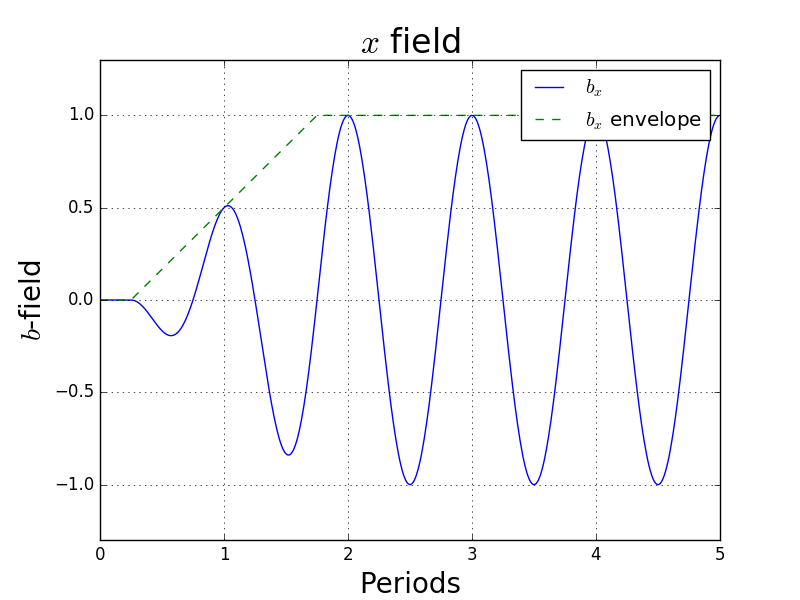
\includegraphics[width=120mm]{bx-field.png}
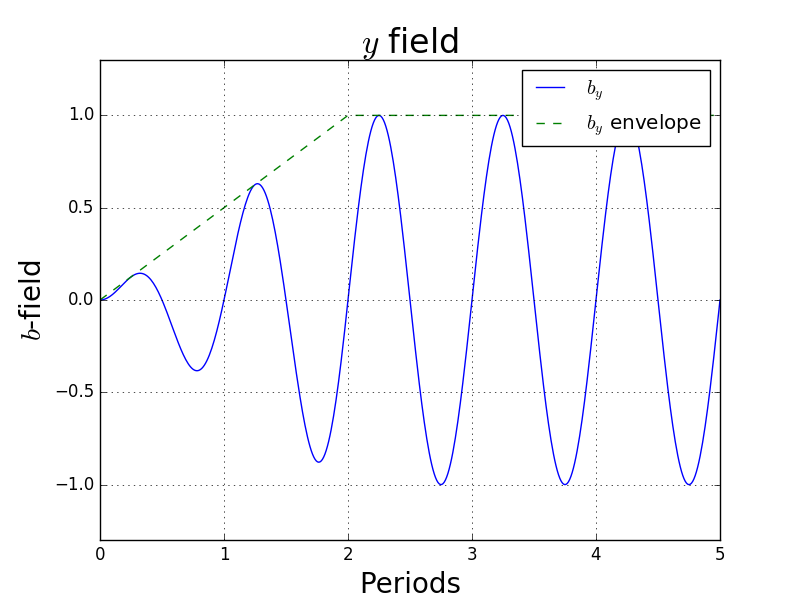
\includegraphics[width=120mm]{by-field.png}
\caption{Schematic of undulator field ends. The magnetic poles are increased linearly over the first 2 periods as shown. }
\label{ends1}
\end{figure*}



Figure \ref{ends1} shows the entry tapers. The $x$ field envelope inceases more rapidly so that the first `pole' is at full strength. The $x$ field is symmetric, and the $y$ field is antisymmetric. The ends of the $x$ field shift the beam off-center by a small amount in the $y$ plane. The $x$ plane motion is not off-set by the $y$ field. Neither causes a velocity offset (or spatial drift) along the undulator. Note that the symmetry of the $x$ field technically results in an extra half-period of full-strength field oscillation in that direction.

These same entry/exit tapers are used for all of the undulator types in Puffin.

% The precise description of the undulator ends are as follows. Note the presence of corrective terms in addition to the main $\cos^2$ term, which ensure the beam oscillates close to the axis. (Note also the very small non-zero initial $z-$magnetic field in each case, which we find  has no noticable deleterious effects in practice.)

%{\bf Helical Front}

%\begin{align}
%b_x  =  \frac{1}{4}\sin(\bar{z}/16\rho) & \cos(\bar{z}/16\rho)    \sin(\bar{z}/2\rho)   +   \sin^2(\bar{z} / 16\rho)  \cos(\bar{z}/2\rho)  \\
%b_y =  - \frac{1}{4}\sin(\bar{z}/16\rho) & \cos(\bar{z}/16\rho)    \cos(\bar{z}/2\rho)   +  \sin^2(\bar{z} / 16\rho)  \sin(\bar{z}/2\rho)\\
%b_z = \frac{\sqrt{\eta}}{2\rho} \Bigl[   \bar{x}\Bigl(& \frac{1}{32}\cos( \bar{z}/8\rho )\sin(\bar{z}/2\rho) +
%           \frac{1}{4}\sin(\bar{z}/8\rho)\cos(\bar{z}/2\rho) \nonumber  \\
%           & - \sin^2(\bar{z}/16\rho)\sin(\bar{z}/2\rho) \Bigr) \nonumber \\
%           \bar{y}\Bigl(& -\frac{1}{32}\cos( \bar{z}/8\rho )\cos(\bar{z}/2\rho) +\frac{1}{4}\sin(\bar{z}/8\rho)\sin(\bar{z}/2\rho) \nonumber  \\
%           & + \sin^2(\bar{z}/16\rho)\cos(\bar{z}/2\rho) \Bigr)  \Bigr]
%\end{align}


%{\bf Helical Back}

%\begin{align}
%b_x  =  -\frac{1}{4}\cos(\bar{z}/16\rho) & \sin(\bar{z}/16\rho)    \sin(\bar{z}/2\rho)   +   \cos^2(\bar{z} / 16\rho)  \cos(\bar{z}/2\rho)  \\
%b_y =  \frac{1}{4}\cos(\bar{z}/16\rho) & \sin(\bar{z}/16\rho)    \cos(\bar{z}/2\rho)   +  \cos^2(\bar{z} / 16\rho)  \sin(\bar{z}/2\rho)\\
%b_z = \frac{\sqrt{\eta}}{2\rho} \Bigl[   \bar{x}\Bigl(& -\frac{1}{32}\cos( \bar{z}/8\rho )\sin(\bar{z}/2\rho) -
%           \frac{1}{4}\sin(\bar{z}/8\rho)\cos(\bar{z}/2\rho) \nonumber  \\
%           & - \cos^2(\bar{z}/16\rho)\sin(\bar{z}/2\rho) \Bigr) \nonumber \\
%           \bar{y}\Bigl(& \frac{1}{32}\cos( \bar{z}/8\rho )\cos(\bar{z}/2\rho) - \frac{1}{4}\sin(\bar{z}/8\rho)\sin(\bar{z}/2\rho) \nonumber  \\
%           & + \cos^2(\bar{z}/16\rho)\cos(\bar{z}/2\rho) \Bigr)  \Bigr]
%\end{align}



%{\bf Plane-Pole Front}

%\begin{align}
%b_x  =  0,  &    \\
%b_y   = \cosh(\sqrt{\eta}\bar{y} / 2\rho)\Bigl[ -\frac{1}{4}& \sin(\bar{z}/16\rho) \cos(\bar{z}/16\rho) \cos(\bar{z} / 2\rho) +   \sin^2(\bar{z}/16\rho) \sin(\bar{z} / 2\rho)   \Bigr], \\
%b_z  =  \sinh(\sqrt{\eta}\bar{y} / 2\rho) \Bigl[ -\frac{1}{32} & \cos(\bar{z}/8\rho) \cos(\bar{z}/2\rho) + \nonumber \\
%                                                &\frac{1}{4}  \sin(\bar{z}/8\rho)\sin(\bar{z}/2\rho) + \sin^2  (\bar{z}/16\rho) \cos(\bar{z}/2\rho)  \Bigr],
%\end{align}

%{\bf Plane-Pole Back}

%\begin{align}
%b_x  =  0,  &    \\
%b_y   = \cosh(\sqrt{\eta}\bar{y} / 2\rho)\Bigl[ \frac{1}{4}& \sin(\bar{z}/16\rho) \cos(\bar{z}/16\rho) \cos(\bar{z} / 2\rho) +   \cos^2(\bar{z}/16\rho) \sin(\bar{z} / 2\rho)   \Bigr], \\
%b_z  =  \sinh(\sqrt{\eta}\bar{y} / 2\rho) \Bigl[ \frac{1}{32} & \cos(\bar{z}/8\rho) \cos(\bar{z}/2\rho) - \nonumber \\
%                                                &\frac{1}{4}  \sin(\bar{z}/8\rho)\sin(\bar{z}/2\rho) + \cos^2  (\bar{z}/16\rho) \cos(\bar{z}/2\rho)  \Bigr].
%\end{align}



%{\bf Curved-Pole Front}


%\begin{align}
%b_x  =  \frac{\bar{k}_{\beta x}}{\bar{k}_{\beta y}} \sinh(\bar{k}_{\beta x} \bar{x})\sinh(\bar{k}_{\beta y} \bar{y}) \Bigl[ -\frac{1}{8}& \sin(\bar{z}/8\rho) \cos(\bar{z} / 2\rho) +   \sin^2(\bar{z}/16\rho) \sin(\bar{z} / 2\rho)   \Bigr],    &    \\
%b_y   =  \cosh(\bar{k}_{\beta x} \bar{x})\cosh(\bar{k}_{\beta y} \bar{y}) \Bigl[ -\frac{1}{8}& \sin(\bar{z}/8\rho) \cos(\bar{z} / 2\rho) +   \sin^2(\bar{z}/16\rho) \sin(\bar{z} / 2\rho)   \Bigr], \\
%b_z  =  \frac{\sqrt{\eta}}{2 \rho \bar{k}_{\beta y}}  \cosh(\bar{k}_{\beta x} \bar{x})\sinh(\bar{k}_{\beta y} \bar{y})  \Bigl[ -\frac{1}{32} & %\cos(\bar{z}/8\rho) \cos(\bar{z}/2\rho) + \nonumber \\
%                                                &\frac{1}{4}  \sin(\bar{z}/8\rho)\sin(\bar{z}/2\rho) + \sin^2  (\bar{z}/16\rho) \cos(\bar{z}/2\rho)  \Bigr] .
%\end{align}

%{\bf Curved-Pole Back}

%\begin{align}
%b_x  =  \frac{\bar{k}_{\beta x}}{\bar{k}_{\beta y}} \sinh(\bar{k}_{\beta x} \bar{x})\sinh(\bar{k}_{\beta y} \bar{y}) \Bigl[ \frac{1}{8}& \sin(\bar{z}/8\rho) \cos(\bar{z} / 2\rho) +   \cos^2(\bar{z}/16\rho) \sin(\bar{z} / 2\rho)   \Bigr],    &    \\
%b_y   =  \cosh(\bar{k}_{\beta x} \bar{x})\cosh(\bar{k}_{\beta y} \bar{y}) \Bigl[ \frac{1}{8}& \sin(\bar{z}/8\rho) \cos(\bar{z} / 2\rho) +   \cos^2(\bar{z}/16\rho) \sin(\bar{z} / 2\rho)   \Bigr], \\
%b_z  =  \frac{\sqrt{\eta}}{2 \rho \bar{k}_{\beta y}}  \cosh(\bar{k}_{\beta x} \bar{x})\sinh(\bar{k}_{\beta y} \bar{y})  \Bigl[ \frac{1}{32} & \cos(\bar{z}/8\rho) \cos(\bar{z}/2\rho) - \nonumber \\
%                                                &\frac{1}{4}  \sin(\bar{z}/8\rho)\sin(\bar{z}/2\rho) + \cos^2  (\bar{z}/16\rho) \cos(\bar{z}/2\rho)  \Bigr] .
%\end{align}




\newpage

\section{Parameters}


Below is an exhaustive list of parameters, for each input file type. Some options are only really useful for investigating runtime errors or strange behaviour. The parameter list for each file is loosely sorted from most to least useful to the average user (default values are in square brackets after the description).


\subsection{Main Input File}

%\begin{lstlisting}[language=fortran]
%sRho
%\end{lstlisting}

All parameters in the main input file are in a single namelist, called {\bf mdata}. They are grouped together below for organisational purposes only.

\subsubsection{Scaling Parameters}

These parameters define the scaling frame used by the Puffin algorithm. The reference wavelength and energies referred to in other parameter descriptions are defined by or derived from these parameters.

{\bf sRho}

$\rho$, the FEL parameter. This specifies the scaling of the system. It does {\bf not} have to be strictly correct - it only descibes the scaling. The simulation can be performed, and the system may be scaled back to SI units, and the result should be correct. If the supplied $\rho$ is correct, however (meaning, it has been calculated from the beam and undulator parameters input), then the scaled notation becomes physically relevant. For an ideal, 1D system, the system should saturate at intensity $|A|^2 \approx 1$, and the system should be firmly in the high or exponential gain regime at $\bar{z} \approx 2-3$. This allows one to quickly see how efficiently the system is lasing w.r.t its ideal case. [$0.01$]

{\bf saw}

$a_u$, the undulator parameter defined with the peak on-axis magnetic field. [$1.0$]

{\bf sgamma\_r}

$\gamma_0$, the reference (usually the mean) beam energy. [$100$]

{\bf lambda\_w}

$\lambda_u$, the undulator, or wiggler, period. [0.04]

{\bf zundType}

Allows one to select from a choice of undulators. Choices are `curved', `planepole', and `helical', described analytically below. If neither of these are chosen, then the default elliptical undulator is chosen, with polarization specified by $u_x$ and $u_y$. [`' (blank - corresponding to the generic variably polarized undulator]

{\bf sux, suy}

$u_x$ and $u_y$ - the relative peak magnetic field of the undulator in each transverse polarization. Usually, at least one should be $=1$, and the other between $0$ (planar) and $1$ (helical). If they are not defined, the default is helical, $u_x=u_y=1$. Ignored if the undulator type is specified as either `helical', `planepole' or `curvedpole'. [($u_x = u_y = 1.0$)]


\subsubsection{Radiation Mesh}

{\bf meshType}

Integer, selecting the mesh type to be used. $= 0$ for fully temporal mesh, $=1$ for periodic mode. [0]

{\bf sperwaves}

Length of the periodic mesh, expressed as the number of reference resonant wavelengths. If {\bf meshType} $=1$ (periodic), and this is defined, then it will be used rather than the more direct {\bf sFModelLengthZ2}. If {\bf meshType} $=1$ then this is ignored. [- (not used by default)] 

{\bf nodesPerLambdar}

Number of nodes in the field mesh to use in the longitudinal dimension per reference resonant wavelength. The reference resonant wavelength is defined from the reference energy {\bf sgamma\_r}, the undulator period {\bf lambda\_w} and the base or reference undulator parameter {\bf saw} in the usual way. [17]

{\bf sFModelLengthZ2}

The full length of the field mesh in the longitudinal or temporal dimension. This must be long enough to contain the entire beam as it propagates through the undulator. It is auto-checked at the start of the simulation for the simple beam case only, and the check is only an estimate. [4.0]

{\bf sFModelLengthX}, {\bf sFModelLengthY}

The full length of the field mesh in the x and y (transverse) dimensions. This must be long enough to contain the entire beam as it propagates through the undulator. It is auto-checked at the start of the simulation for the simple beam case only, and the check is only an estimate. [1.0, 1.0]

{\bf iNumNodesX, iNumNodesY}

Number of nodes in the field mesh in the $x$ and $y$ transverse dimensions, respectively. [129,129]

{\bf iRedNodesX, iRedNodesY}

If {\bf qFixMesh} $=$ {\bf .true.}, then the mesh size in $x$ and $y$ will be altered in the initialization stage so that the inner {\bf iRedNodesX} $\times$ {\bf iRedNodesY} nodes in the transverse plane contain the beam. Only works for the simple beam input type. [20,20 (won't be fixed)]

{\bf nspinDX, nspinDY}

Inner set of transverse nodes to be used in the MPI process updates, which should contain the full transverse beam - auto-calculated in Puffin if wrong. [20,20]

{\bf seed\_file}

String - name of the radiation seed input file. [`' (blank string)]

\subsubsection{Electron Beam}


{\bf beam\_file}

String - name of the electron beam input file. [`beam\_file.in']

{\bf sElectronThreshold}

When using the simple beam generation, any macroparticles generated with weight below the threshold will be removed. The threshold is defined using this variable, which expresses the threshold as a percentage of the mean particle weight. [0.05]


\subsubsection{Undulator Lattice}

{\bf lattFile}

The name of the lattice file, if required. If not required, supply a blank string (enter {\bf `'}). [`' (blank string)]

{\bf nPeriods}

Number of undulator periods in the single (non-lattice) undulator case. If a lattice file is suppiled, then this is ignored. [8]

{\bf taper}

Taper in the single, simple undulator case, $\dfrac{d\alpha}{d \bar{z}}$. Ignored if a lattice file is supplied. [$0.0$]

{\bf sKBetaXSF, sKBetaYSF}

Betatron wavenumber for energy $\gamma_r$ of the applied strong focussing channel over the wiggler. Ignored if {\bf qFocussing} is {\bf .false.}. Both $=0$ if not specified. Remember this will be applied on top of wiggler field, which has it's own natural focussing. [0.0, 0.0]

\subsubsection{Data Writing Options}

These options control the frequency of the writing of the output data files.

{\bf iWriteNthSteps}

Steps at which to write the full data dumps at. This sets the periodicity of the data dumps, in integration steps. [$30$]

{\bf iWriteIntNthSteps}

Steps at which to write the integrated data at. This sets the periodicity of the writes, in integration steps. [$30$]

{\bf qInitWrLat}

Logical. If true, there will be a full particle and field mesh dump at the end of each undulator module in the lattice, and the writing counter will be reset. [.false.]

{\bf qDumpEnd}

Logical. If true, write a full data dump at the end of the simulation, even if it does not occur at an integer number of {\bf iWriteNthSteps}. [.true.]




\subsubsection{Options}

{\bf qOneD}

Logical. If  {\bf .true.}, Puffin will be run in 1D mode. Default is  {\bf .true.}, since this is the least computationally expensive option. [.true.]

{\bf qFieldEvolve}

Logical. If = {\bf .false.}, then the radiation field evolution will be switched off. This is obviously artificial and very rarely used, but can be useful for debugging in some instances. Default is = {\bf .true}. [.true.]

{\bf qElectronsEvolve}

Logical. If = {\bf .false.}, then the electron equations are not solved in the integration steps. Like the case when qFieldEvolve= {\bf .false.},  this is obviously artificial and very rarely used, but can be useful for debugging in some instances. Default is = {\bf .true.}. [.true.]

{\bf qElectronFieldCoupling}

Logical. If = {\bf .false.}, then the radiation field feedback onto the electrons is switched off by setting the field terms in the electron evolution equations = 0, and so switches off the amplification of the radiation from the electrons. This is unphysical, but is used more often than when qFieldEvolve and qElectronsEvolve ={\bf .false.} . It can often be used to check for gain in the FEL in low gain situations, or to check whether amplification has occurred rather than coherent emission (CSE) effects due to \textit{e.g.} fine structure in the beam. When ={\bf .false.}, this will give the purely spontaneous emission (coherent or incoherent) from the electrons in the wiggler. If there is no appreciable difference between the qElectronFieldCoupling=true and false cases, then there has been negligible FEL amplification. [.true.]

{\bf qSeparateFiles}

If each rank is writing its own file for the hdf5 files. If = true, then the files will need to be gathered together in post for analysis. Depending on the file system, this may be faster or slower for you. There are some post-processing python scripts to show how you might stitch the files together in post. [.false.]

{\bf qFocussing}

Allows one to switch the strong focussing channel on or off. If ={bf .true.}, the strong focusing is switched on with calues specified by sKBetaXSF and sKBetaYSF. If qFocussing={\bf .true.}, yet no focussing strength is specified (sKBetaXSF or sKBetaYSF), then strong focusing is effectively switched off in that dimension. Default = {\bf .false.}. [.false.]

{\bf qDiffraction}

Switches modelling of diffraction of the radiation field on or off. If ={\bf .true.}, field diffraction is modelled. This can be useful to switch off only really for debugging purposes. Default ={\bf .true.}. [.true.]

{\bf qFMesh\_G}

Whether fixing the field mesh in the transverse plane to contain the beam within the inner {\bf iRedNodesX} $\times$ {\bf iRedNodesY} nodes. Valid when using a `simple' beam only - otherwise it is ignored. [.true.]

{\bf qUndEnds}

Switch on/off proper modelling of the wiggler module ends. If true, then the first and last 2 periods of the wiggler will be tapered up/down with a $\sin^2$ function. [.false.]

{\bf q\_Noise}

If adding the statistical shot-noise to the beam in the simple beam case. [.true.]

{\bf qsdds}

Switch on/off ouput of particle and field mesh dumps in sdds format. [.false.]

{\bf qhdf5}

Switch on/off output of particle and field mesh dumps in vizSchema compliant hdf5 format. [.true.]

{\bf qScaled}

Logical turning on/off the input of scaled units into Puffin. If {\bf .true.}, input is assumed to be in the scaled units. [.true.]

{\bf qFilter}

Logical turning on/off the filtering of low frequency content during the siffraction step. The high-pass filter cut-off is defined by {\bf sFiltFrac}. If true, the low frequency content is set $=0$. If false, the low frequency content is not manipulated/diffracted. [.true.]

{\bf qWriteA, qWriteZ2, qWritePperp, qWriteP2, qWriteX, qWriteY, qWriteZ}

Logicals to switch on/off the writing of field, electron phase space coordinates ($\bar{z}_2$, $\bar{p}_\bot$, $\Gamma$, $\bar{x}$, $\bar{y}$), and propagation distance, respectively, in the sdds full data dumps. (Deprecated) (Only used when {\bf qsdds = .true.})

\subsubsection{Numerical Integration}

These parameters control the numerical integration methods.

{\bf stepsPerPeriod}

Number of integration steps for the electron beam and field source term per undulator period. Should usually be $\gtrsim$ {\bf nodesPerLambdar} for a beam with energy and wiggler parameter close to the reference parameters. [30]

{\bf sDiffFrac}

Length of the diffraction step, in units of the undulator period. Usually $=1$. [1.0]

{\bf sFiltFrac}

During the field diffraction step, the lower frequencies are filtered out. This sets the cutoff for the high-pass filter, in units of the reference resonant frequency - (so should usually be $\leq 0.3$). [0.3]

{\bf sBeta}

Absorption coefficient for the absorbing boundaries on the transverse grid. [1.0]

{\bf sRedistLen, iRedistStp}

Parallel tuning parameters, controlling the buffer length needed by each MPI process, and the number of steps per redistribution stage, respectively. [4.0, 60]

\newpage

\subsection{Beam Input File}

As noted in section \ref{beamfls}, the electron beam can be specified in 3 different forms - either a `simple', `dist' or `particle'.

The beam file must contain $2$ namelists. One to choose the method, and the other to choose the options particular to that method. To choose which method to use, the beam file first of all contains a namelist titled {\bf nblist} with the following parameters.

\subsubsection{Namelist: nblist}

{\bf dtype}

String, specifying type of beam input. Can be either {\it simple}, {\it dist} or {\it h5} (for particle input type)

{\bf nbeams}

Integer. The number of electron beams to set up. For a simple beam, multiple beam can be setup. For the dist type input, multiple electron beam dist files can be used. For the particle input, this parameter is ignored.

If {\bf dtype} $=$ {\it simple}, then a namelist called {\bf blist} must be used, if {\bf dtype} $=$ {\it dist} the namelist {\bf bdlist} must be entered, and if {\bf dtype} $=$ {\it h5} the namelist {\bf bh5list} must be entered.

\subsubsection{Namelist: blist}

For the simple beam file, one can set up a homogeneous beam in every dimension. Some additional manipulation can be made to this simple beam with the supplied options - Twiss parameters can be used, or a simple beam energy modulation. The beam is assumed to have either a Gaussian or flat-top distribution profile in each dimension. The beam is therefore specified by giving the widths and so forth of the beam.

{\bf sSigmaE}





% simple params:
%
%sSigmaE, sLenE, iNumElectrons, &
%                   sEmit_n, sQe, bcenter,  gammaf, &
%                   chirp, mag, fr, qRndEj_G, sSigEj_G, &
%                   qMatched_A, qEquiXY, nseqparts, qFixCharge, &
%                   alphax, alphay, emitx, emity, TrLdMeth, fillFact





\newpage

\subsection{Radiation Seed Input File}

The seed file can be in 2 forms - one describing a homogeneous seed of Gaussian or flat top profiles in each of the 3 spatial directions, or a list of hdf5 files containing the values of the $x$ and $y$ fields at the nodes of the radiation mesh.

As with the beam file, the seed file contains 2 namelists - one specifying which of the 2 input methods is being used and the number of seeds, and the other containing the specification for the selected method.


\newpage

\subsection{Lattice File}

The main input file allows one to descibe a single undulator. The lattice file instead allows one to construct a more sophisticated layout for the FEL beam line, incuding multiple undulator modules, focussing quadrupoles, drift sections, simple beam modulator sections and chicanes. If the lattice file is given, the single undulator in the main input file is ignored.

An example of a lattice file is given below. Each lattice element is described by a single line of the lattice file. For a line to be read as a lattice element, it must begin with a two letter (all caps) identifier corresponding to a lattice element. Any line not beginning with a legal identifier is ignored.

\lstset{style=mystyle}
\begin{lstlisting}[language=fortran, caption=Example lattice file.]
!Module file for Puffin
!CLARA lattice v3 - reduced for example
!This is for using undulator ends to give
!25 'active' undulator periods.
!The drift is calculated to give a strict 1.25m
!distance between quads
!A small (currently dispersionless) phase shifter is used to knock the beam
!back to the correct phase after the drift.

QU -4.78 4.78

UN  'planepole'  29   1.0   0.0   30   1.0   1.0   0.0    0.0
DR 16.4545455
CH  0.0  0.966  0.0
QU 2.39 -2.39

UN  'planepole'  29   1.0   0.0   30   1.0   1.0   0.0    0.0
DR 16.4545455
CH  0.0  0.966  0.0
QU -2.39 2.39

UN  'planepole'  29   1.0   0.0   30   1.0   1.0   0.0    0.0
DR 16.4545455
CH  0.0  0.966  0.0
QU 2.39 -2.39

UN  'planepole'  29   1.0   0.0   30   1.0   1.0   0.0    0.0
DR 16.4545455
CH  0.0  0.966  0.0
QU -2.39 2.39

UN  'planepole'  29   1.0   0.0   30   1.0   1.0   0.0    0.0
DR 16.4545455
CH  0.0  0.966  0.0
QU 2.39 -2.39

\end{lstlisting}

Each identifier is then followed by a series of parameters to specify the element's variables. For the undulator element:

\begin{lstlisting}[language=fortran, caption=Undulator identifier and specification]
UN  'planepole'  29   1.0   0.0   30   1.0   1.0   0.0    0.0
! The parameters following the identifier are:
zundtype, nw, mf, taper, nperlam, ux_arr, uy_arr, kbnx_arr, kbny_arr
!
! zundtype is a string describing the undulator type. Choose from 'helical', 'planepole', 'curved', or '' (blank string)
!
! nw is an integer giving the number of periods in this undulator
!
! alpha is a float giving the initial undulator tuning for this module aw/aw0,
!
! taper is the undulator magnetic field taper d/dz of alpha (float)
!
! nperlam is an integer specifying the number of integration steps per undulator period to be used in this undulator
!
! ux and uy - relative magnetic field strengths in x and y, respectively (float)
!
! kbnx_arr and kbny_arr - betatron wavenumber (k_beta = 2pi / lambda_beta)
! of constant 'strong' focusing channel applied over undulator (float)
\end{lstlisting}

Focusing quads are modelled as a simple point transform, see section \ref{latt-file}.

\begin{lstlisting}[language=fortran, caption=Quadrupole identifier and specification]
QU 2.39 -2.39
! Parameters being \bar{F}_x and \bar{F}_y, which are F_x / lg and Fy / lg, respectively. (F_x being -1/R21 of
! the quad transport matrix, and F_y being -1/R43).

\end{lstlisting}



%! zundtype_arr, nw, mf, tapers, nperlam, ux_arr, uy_arr, kbnx_arr, kbny_arr
%!
%! ...being...
%!
%! undulator type, number of periods (integer), initial tuning alpha = aw/aw0,
%! taper d/dz alpha, number of integration steps per undulator period (integer),
%! ux and uy - relative magnetic field strengths in x and y, respectively
%! kbnx_arr and kbny_arr - betatron wavenumber (k_beta = 2pi / lambda_beta)
%! of constant 'strong' focusing channel applied over undulator

\newpage

\subsection{Write File}

The seed file can be in 2 forms - one describing a homogeneous seed of Gaussian or flat top profiles in each of the 3 spatial directions, or a list of hdf5 files containing the values of the $x$ and $y$ fields at the nodes of the radiation mesh.

As with the beam file, the seed file contains 2 namelists - one specifying which of the 2 input methods is being used and the number of seeds, and the other containing the specification for the selected method.



\newpage

\begin{thebibliography}{10}

\bibitem{puffin}
L.T. Campbell and B.W.J. McNeil, Physics of Plasmas {\bf 19}, 093119 (2012)
\bibitem{2col}
L T Campbell, B.W.J. McNeil and S. Reiche, New J. Phys. {\bf 16} (2014) 103019
\bibitem{scharlemann1}
E.T. Scharlemann, in High Gain, High Power FELs (edited by R. Bonifacio \textit{et al} ) (1989)
\bibitem{noise1}
B. W. J. McNeil, M. W. Poole, and G. R. M. Robb, Phys. Rev. ST Accel. Beams {\bf 6}, 070701 (2003)


\end{thebibliography}

\end{document}
